\chapter{Results}\label{ch:results}
Presented here are a number of test cases which access the accuracy of the matrix exponential solvers in libowski. The majority of analysis thus far is done on what is known as Problem 1. Two major properties which influence the accuracy of each method are exploited, matrix norm and eigenvalues with both time stepping methods. There are also verification problems for diffusion and convection problems to test the spatial and temporal accuracy. Finally there is a neutron precursor problem showing the application in a nuclear reactor type test problem. 

As a comparison, the classical numerical ODE integration method backward differentiation formula (BDF) of various orders are also used to solve the practice problems. BDF integrators are a class of implicit multistep methods used for stiff differential equations. 

\section{TVD Convective Flux}
Implementation of the deferred corrections second order flux for a number of flux limiting function is assessed with a number of test problems. Each of these problems consist of solving the following PDE,

\begin{equation}
    \frac{\partial \rho}{\partial t} = -v\frac{\partial \rho}{\partial x},
\end{equation}

\noindent with various initial and boundary conditions. 

\section{Matrix Exponential Accuracy}
\subsection{Problem 1}
This test contains two variations of the same three isotope decay problem shown in Equation \ref{eq:problem1}. In each problem, the decay constants are changed to induce different eigenvalues.

\begin{equation}
\begin{split}
    \frac{dN_{1}}{dt} &= \lambda_{3}N_{3} - \lambda_{1}N_{1}, \quad N_{1}(0) = 10000\\
    \frac{dN_{2}}{dt} &= \lambda_{1}N_{1} - \lambda_{2}N_{2}, \quad N_{2}(0) = 0\\
    \frac{dN_{3}}{dt} &= \lambda_{2}N_{2} - \lambda_{3}N_{3}, \quad N_{3}(0) = 0
\end{split}
    \label{eq:problem1}
\end{equation}

Problem 1a induces only real eigenvalues $[0, -0.02, -0.025]$ and $||A||_{l_{1}} =0.06$ when $t=1$ and linearly increases to $36$ when $t_{end}=600$. The corresponding decay constants are $[\lambda_{1}, \lambda_{2}, \lambda_{3}] = [0.1, 0.005, 0.03]$. Both time marching methods are tested against an analytical solution which was generated in Matlab. 


Results for time marching scheme 1 were generated by taking one time step to $t_{end} = 600$. Table \ref{tab:results1a} shows that the Hyperbolic solver outperforms all other solvers for isotopes 2 and 3 while performs as well as the CRAM solver for isotope 1. Both Pad\'e methods gives the same $l_{\infty}$ error for each isotope and is only slightly larger than the minimum error for isotope 1. The Parabolic solver has the worst error for all isotopes. 

Test are conducted with time marching scheme 2 at various time steps for each solver. The $l_{\infty}$ error for each isotope are is shown in Figure \ref{fig:errorProblem1aTimeMarchingScheme2} for the exponential solvers and Figure \ref{fig:errorProblem1aTimeMarchingScheme2Int} for the BDF solvers. Error for each of the Cauchy solvers exponentially decays as you decrease the number of substeps (increase the time step size) you take as your march to $t_{end}=600$. Because the isotope concentrations do not sharply decrease as steady state is reached, substeping a Cauchy solver will not increase the accuracy. The reason the accuracy decreases was described in Section \ref{sec:timeMarchingSchemes}. In general, the Pad\'e solvers also follow this trend although it is not as sharp as the Cauchy solvers. Pad\'e-Method 1 shows a sharp increase in error after the first time step size then tends to decrease with few small increases in error between a number of time steps. These small increases might be caused by the matrix norm increases but not enough to jump to a higher order Pad\'e function. When the norm increases over that Pad\'e orders threshold, the error sharply jumps down because a higher order Pad\'e method is used to approximation the matrix exponential. After a point the matrix norm becomes too large, and squaring a scaling takes place. 

In general, the BDF solvers show sporadic behavior for large time steps with very high error. BDF of orders greater than 2 are not A-stable which might answer why some of the errors are quite large for the larger time steps with high order BDF's. In BDF orders 2, 3, 5 and 6 the first few points have lower error where the number of points corresponds to the BDF order - 1. This behavior comes from the way in which the initial points are calculated to start the BDF solver. For example, BDF5 requires 5 previous solutions to compute the next point, therefore 4 previous solutions need to be calculated to start the solver. These previous solutions are calculated with a much finer time step size and with lower order BDF's, to not introduce error at the beginning of the solution. After the number of steps increases to the order of the requested BDF method then the actual BDF method kicks in and starts to compute the solution. After each solver begins running with higher and higher time steps, you can see the slope of the error vs time step size corresponding to the order of each solver. As you increase the BDF order the slope increases, showing faster convergence for higher order methods. What is most notable about comparing the BDF solvers with the exponential ones is the difference in relative accuracy. The worst preforming exponential solver beat the best preforming BDF method and their accuracy vs time step size are inversely proportional to one another. Meaning that the exponential solvers preform better with a single time step than with multiple, which was discussed earlier. The take away from this comparison is that the exponential solvers far outpreformed the BDF methods. 

\begin{table}[b]
    \caption{\label{tab:results1a} Problem 1a $l_{\infty}$ Error for Time Marching Scheme 1}
    \centering
    %\begin{tabular}{c|p{1.5cm}|p{1.5cm}|p{1.5cm}|p{1.5cm}|p{1.5cm}|p{1.5cm}}
    \begin{tabular}{c|c|c|c}
    \hline
     & $N_{1}$ & $N_{2}$ & $N_{3}$ \\
    \hline
    \hline
    CRAM & 7.28E-12 & 5.46E-12 & 2.39E-12 \\
    \hline
    Parabolic & 6.37E-11 & 6.46E-11 & 2.40E-11 \\
    \hline
    Hyperbolic & 7.28E-12 & 4.09E-12 & 1.40E-12 \\
    \hline
    Pad\'e Method 1 & 7.73E-12 & 1.27E-11 & 2.16E-12 \\
    \hline
    Pad\'e Method 2 & 7.73E-12 & 1.27E-11 & 2.16E-12 \\
    \hline
    \end{tabular}
\end{table}

\begin{figure}[t]
  \centering
  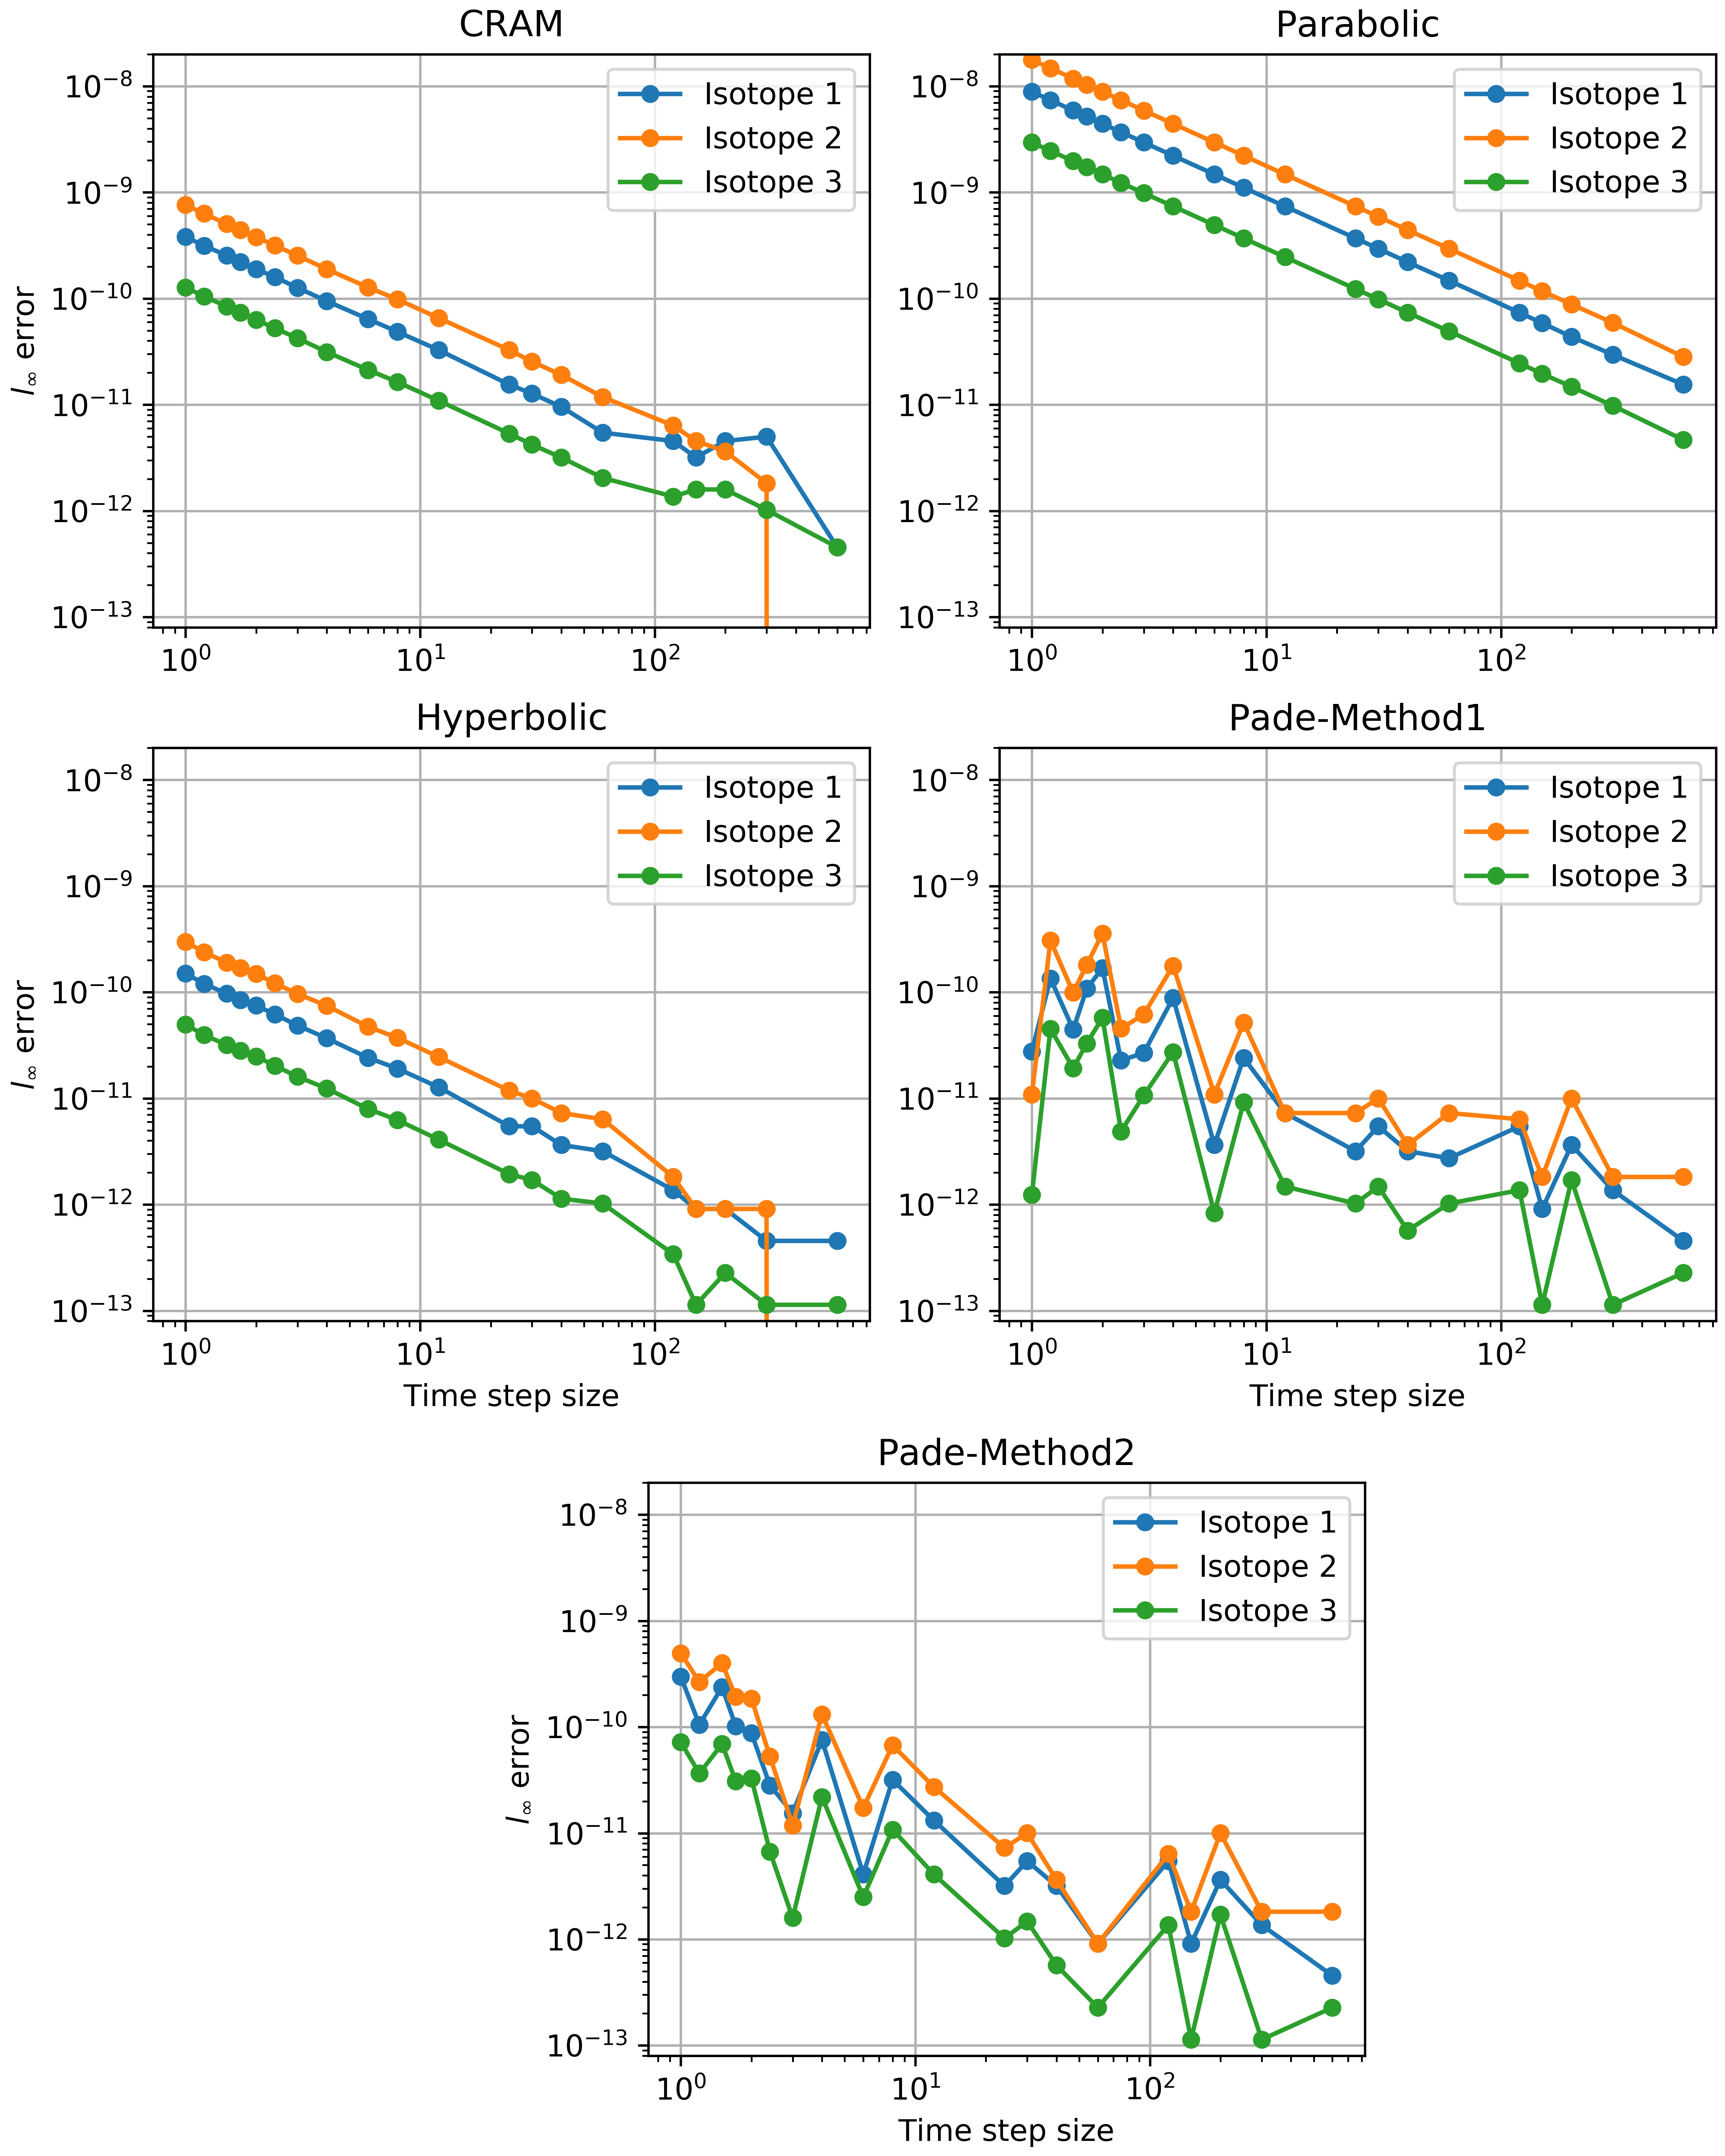
\includegraphics[width=6.5in]{images/problem1aMethod2.png}\\
  \caption{Error for Problem 1a Using Time Marching Scheme 2 with Exponential Solvers}
  \label{fig:errorProblem1aTimeMarchingScheme2}
\end{figure} 

\begin{figure}[t]
  \centering
  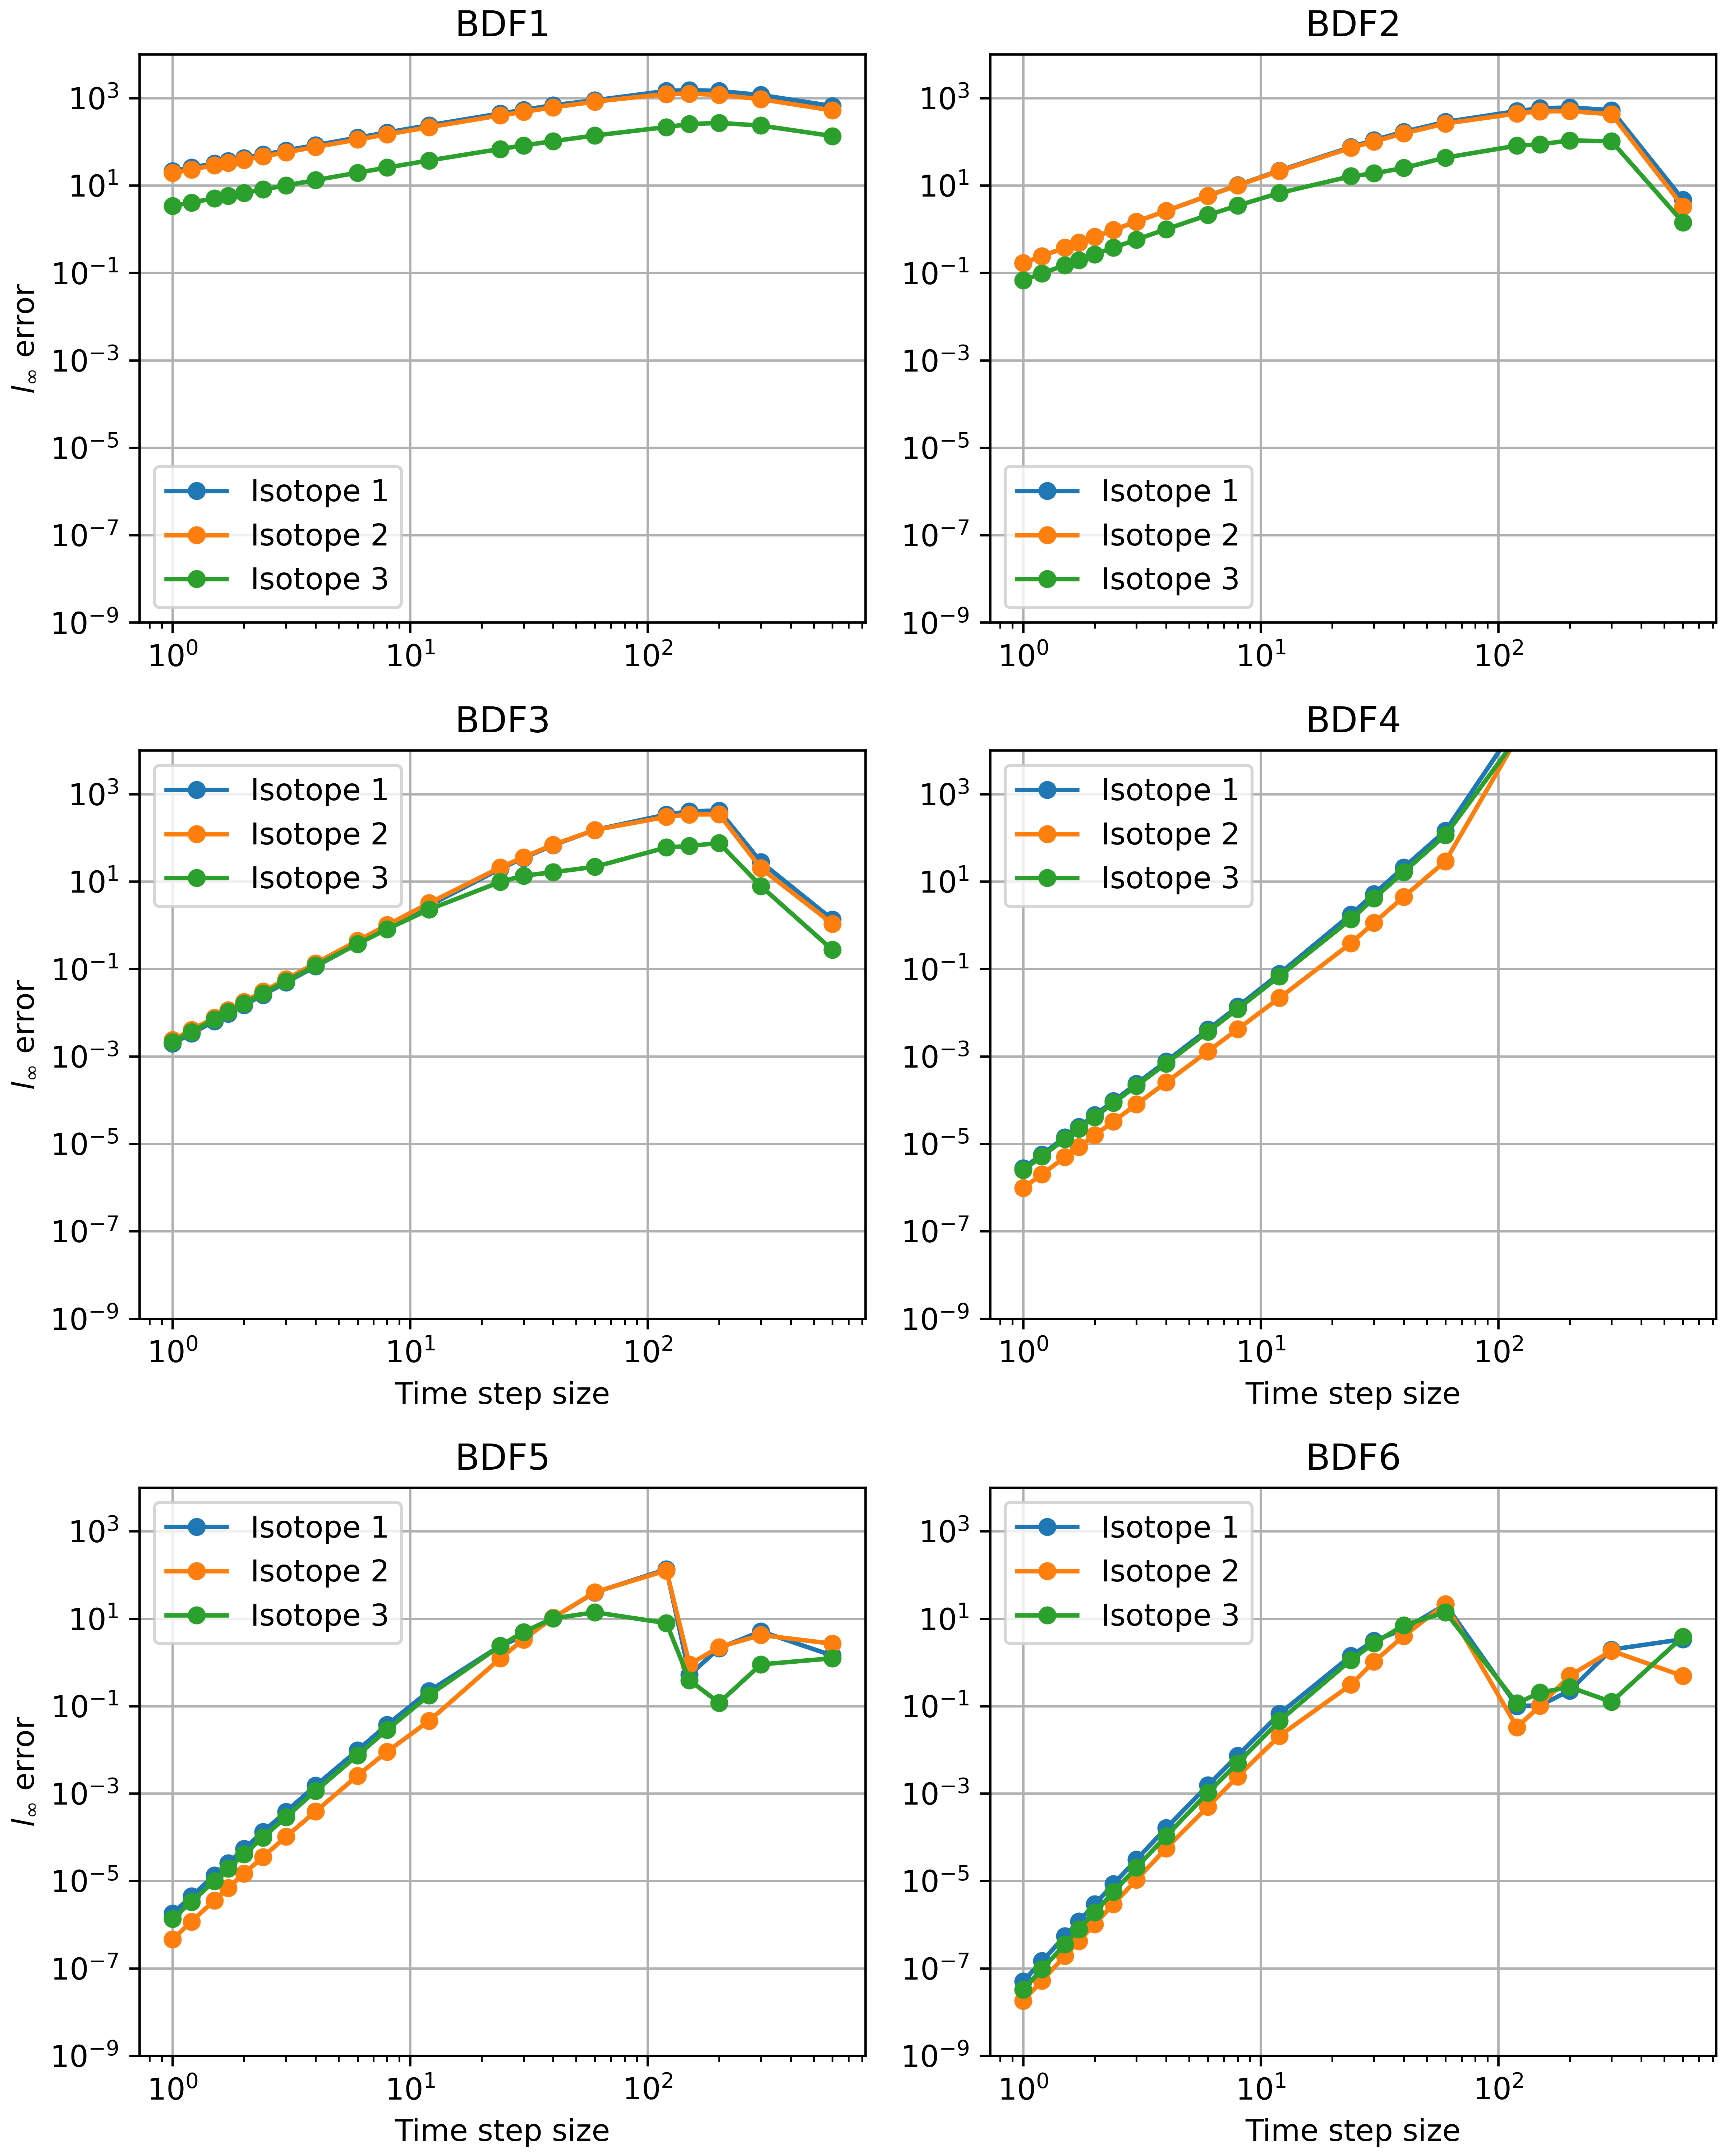
\includegraphics[width=6.5in]{images/problem1aMethod2Int.png}\\
  \caption{Error for Problem 1a Using Time Marching Scheme 2 with BDF Solvers}
  \label{fig:errorProblem1aTimeMarchingScheme2Int}
\end{figure} 

\FloatBarrier



Problem 1b modifies the decay constants to produce eigenvalues with imaginary parts [2.05e-19, -1.5e-02+0.00707107i, -1.5e-02-0.00707107i] with $||A||_{l_{1}} = 0.03$ when $t=1$ and linearly increases to 18 when $t_{end} = 600.$ The corresponding decay constants are $[\lambda_{1}, \lambda_{2}, \lambda_{3}] = [0.1, 0.005, 0.105]$. Again, the solution was generated in Matlab. 

Results for time marching scheme 1 were generated by taking one time step to $t_{end} = 600$. Table \ref{tab:results1b} shows that CRAM was the worst preforming solver. This is not surprising considering the magnitude of the imaginary parts of the eigenvalues, CRAM is most accurate around the negative real axis. Both Parabolic and Hyperbolic solvers cover a wider range on the imaginary axis, which shows in the results. Each of these solvers are many orders of magnitude more accurate than CRAM. The Pad\'e solvers both give the same solution, this is not surprising because there are situations in Pad\'e Method 2 which will run as Method 1. Again the Hyperbolic solver is the most accurate.

Results for time marching scheme 2 are shown in Figure \ref{fig:errorProblem1bTimeMarchingScheme2} and shows one of the advantages of substepping. As the time step length increases, so do the placement of the eigenvalues on the complex plane. If the time step is too large, the eigenvalues can shift into a region which decreases the accuracy of Cauchy methods; this behavior is most prevalent in CRAM. Both the Parabolic and Hyperbolic solvers also show a slight bump in error after time steps on the order of 100, after the error starts to decline again and bottoms out at the last point. The last point corresponds to taking a single time step. Both of the Pad\'e solvers show the same general trend as with problem 1a. The matrix norm for this problem is slightly lower than with problem 1a, leading to lower error. Figure \ref{fig:errorProblem1bTimeMarchingScheme2Int} shows the error for the BDF methods. The error for each order shows the same general behavior as with problem 1b. A notable exception to this is BDF4, which shows greater accuracy for low number of time steps. Again, the exponential methods out preform the BDF integrators. 

\begin{table}[b]
    \caption{\label{tab:results1b} Problem 1b $l_{\infty}$ Error for Time Marching Scheme 1}
    \centering
    %\begin{tabular}{c|p{1.5cm}|p{1.5cm}|p{1.5cm}|p{1.5cm}|p{1.5cm}|p{1.5cm}}
    \begin{tabular}{c|c|c|c}
    \hline
     & $N_{1}$ & $N_{2}$ & $N_{3}$ \\
    \hline
    \hline
    CRAM & 5.73E-9 & 4.37E-9 & 1.36E-9 \\
    \hline
    Parabolic & 8.64E-11 & 9.09E-12 & 1.26E-10 \\
    \hline
    Hyperbolic & 9.09E-13 & 9.09E-13 & 6.82E-13 \\
    \hline
    Pad\'e Method 1 & 1.36E-12 & 9.09E-13 & 2.27E-13 \\
    \hline
    Pad\'e Method 2 & 1.36E-12 & 9.09E-13 & 2.27E-13 \\
    \hline
    \end{tabular}
\end{table}

\begin{figure}[t]
  \centering
  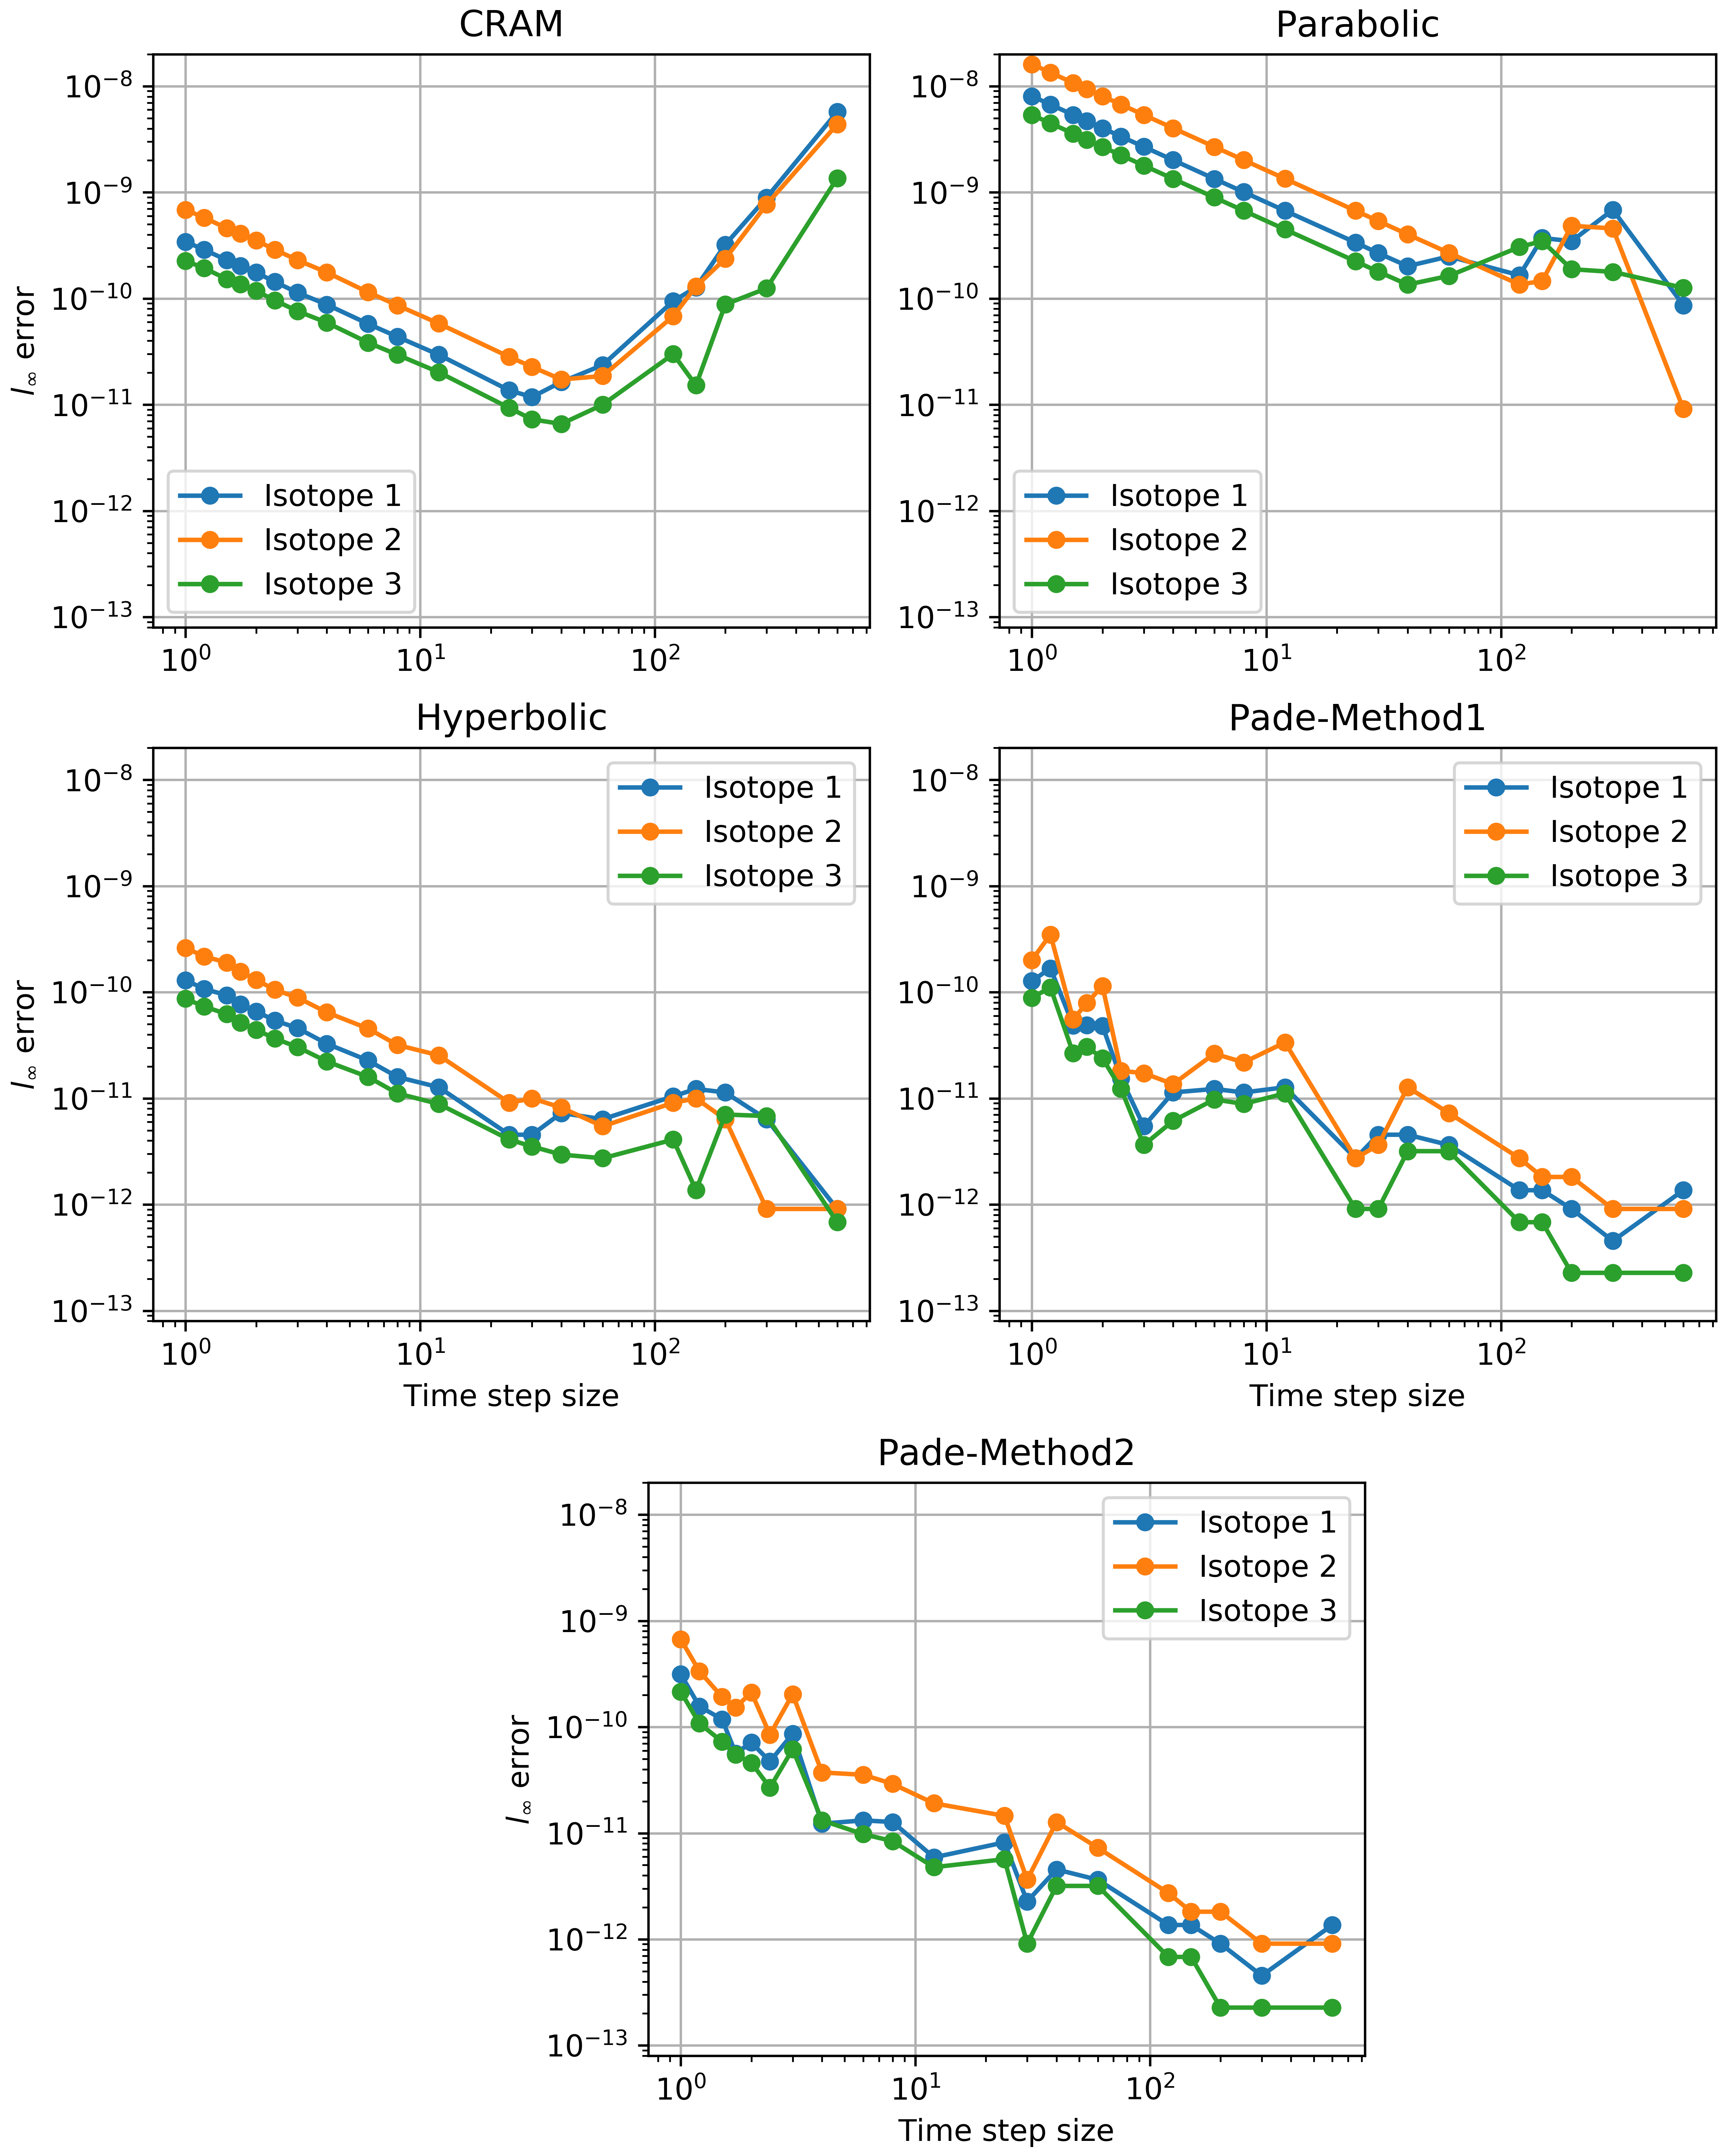
\includegraphics[width=6.5in]{images/problem1bMethod2.png}\\
  \caption{Error for Problem 1b Using Time Marching Scheme 2 with Exponential Solvers}
  \label{fig:errorProblem1bTimeMarchingScheme2}
\end{figure} 

\begin{figure}[t]
  \centering
  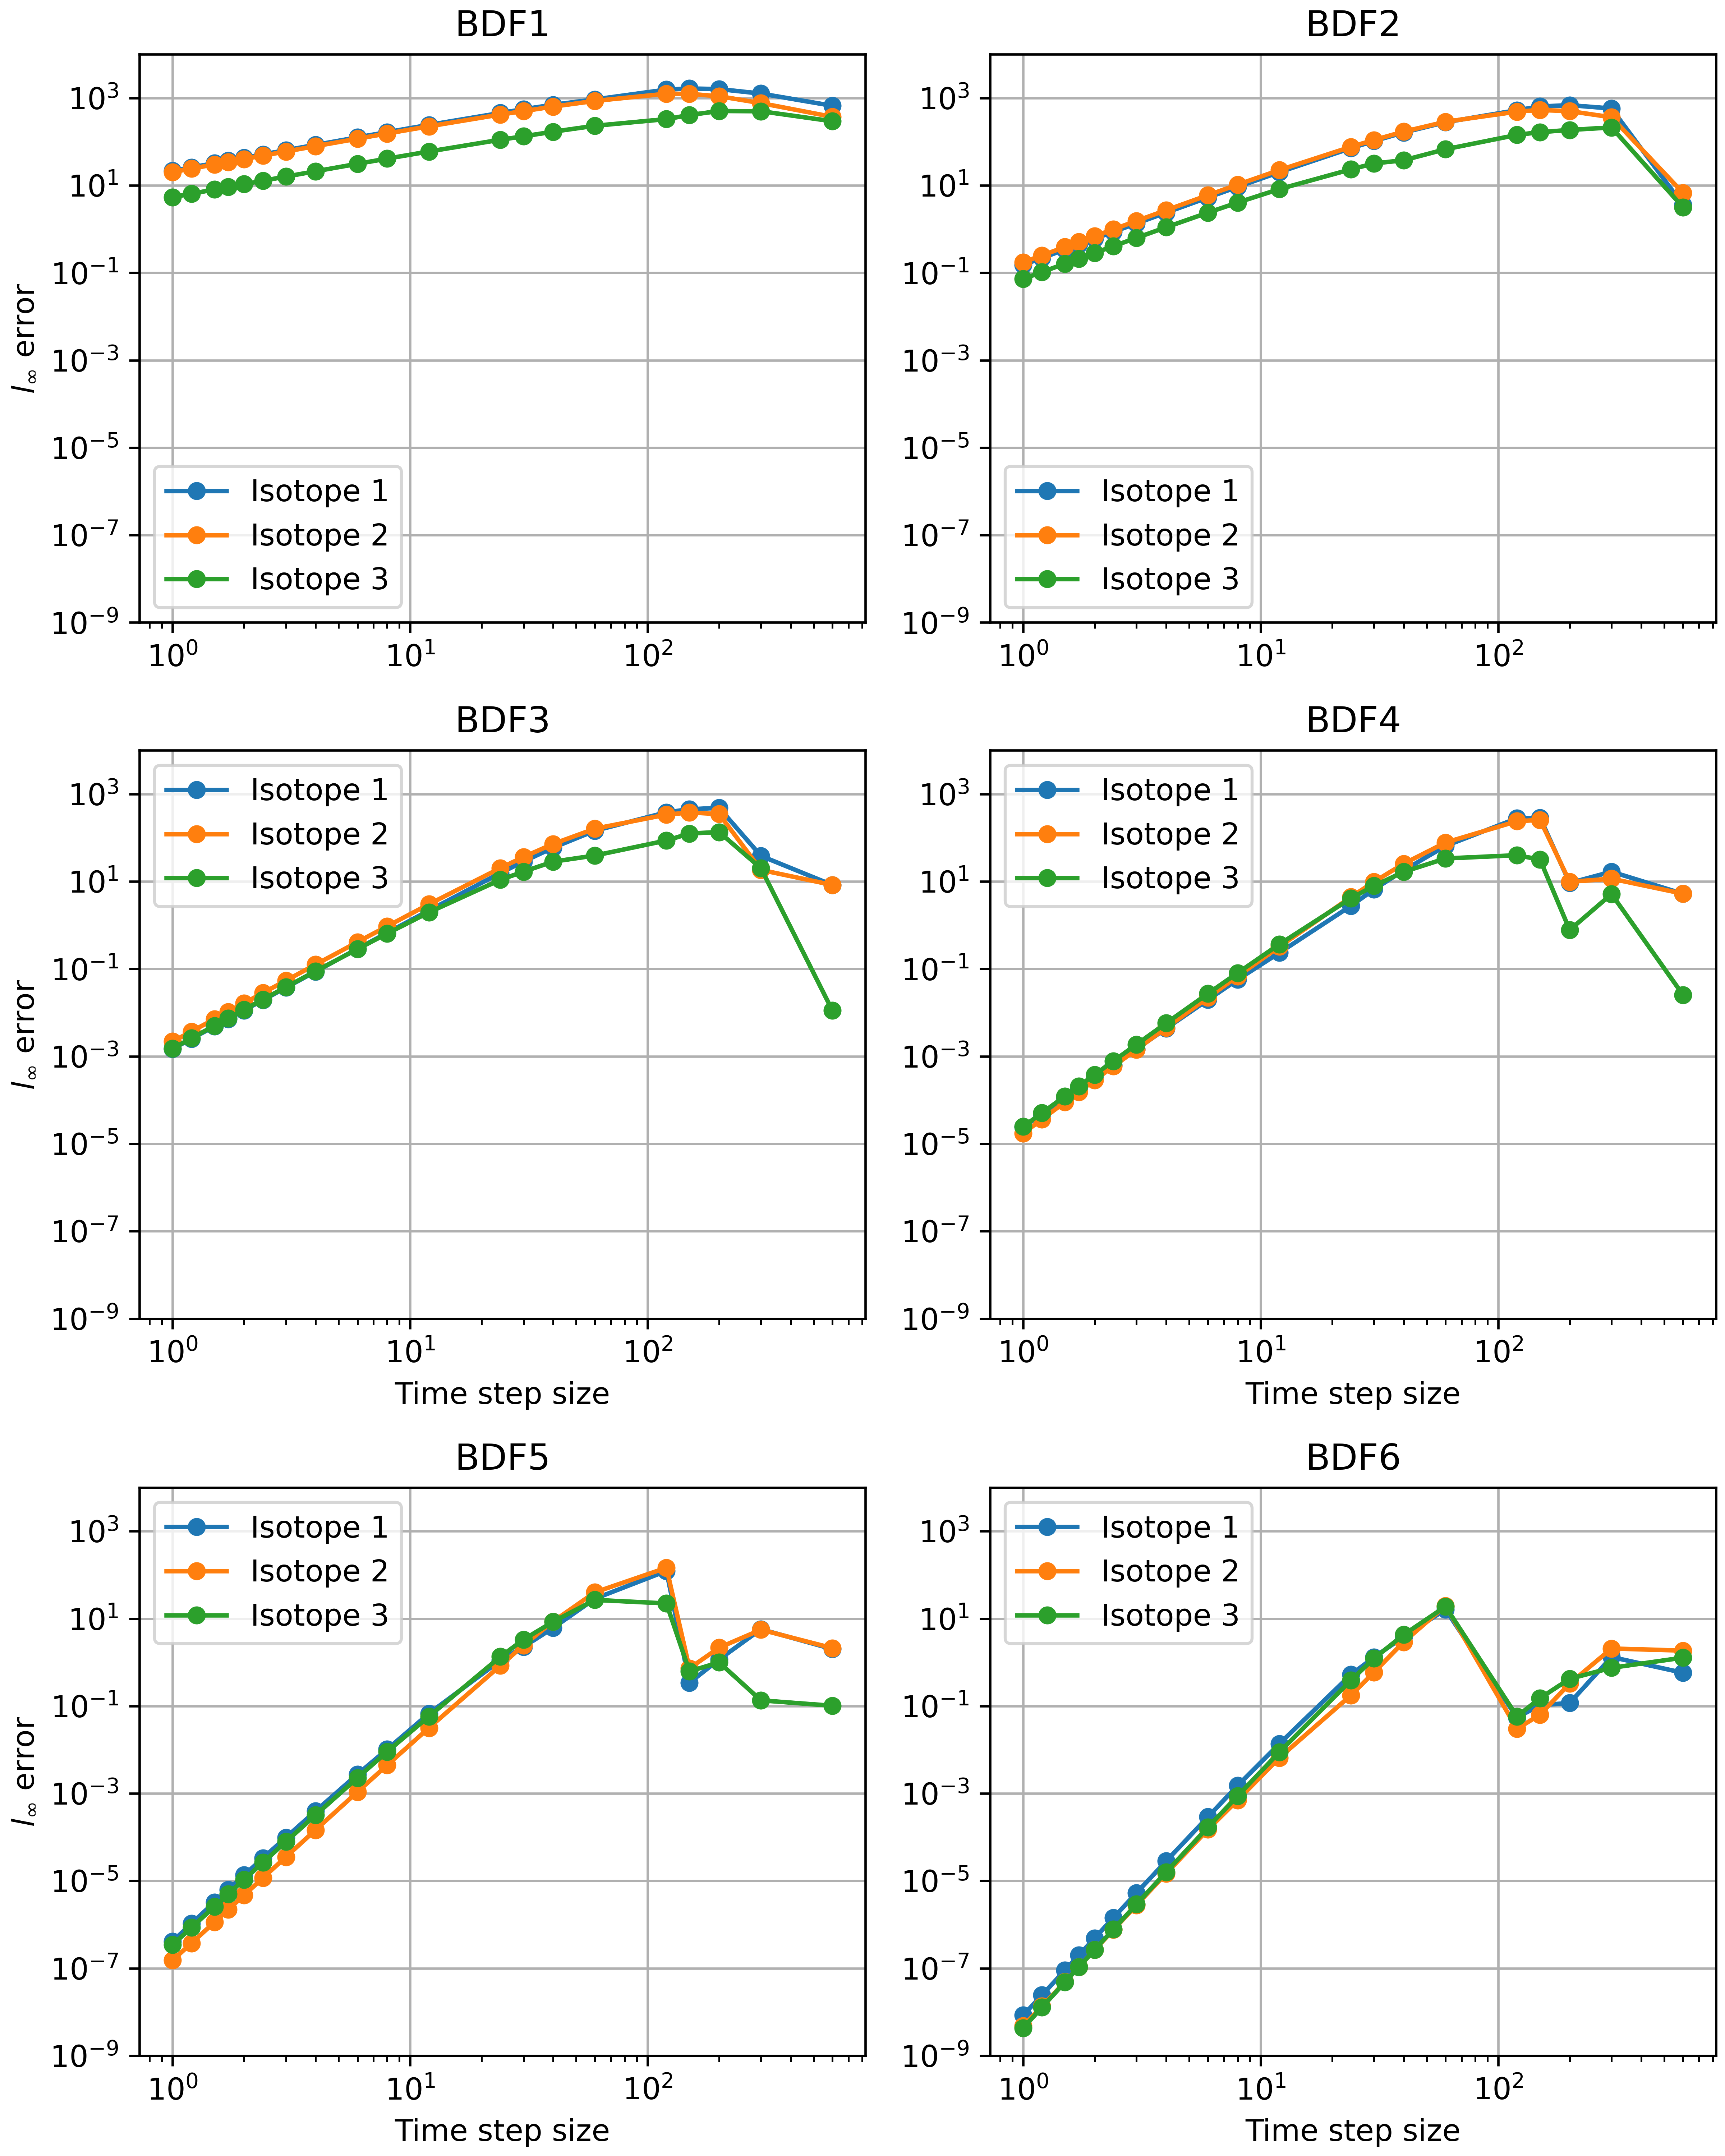
\includegraphics[width=6.5in]{images/problem1bMethod2Int.png}\\
  \caption{Error for Problem 1b Using Time Marching Scheme 2 with BDF Solvers}
  \label{fig:errorProblem1bTimeMarchingScheme2Int}
\end{figure} 

\FloatBarrier

\subsection{Problem 2}
Problem 2 is a 1D, two species reaction-diffusion problem shown in Equation \ref{eq:problem2Eqs} \cite{ching2007},

\begin{equation}
\setlength{\jot}{15pt}
\begin{split}
    \frac{\partial U}{\partial t} &= d\frac{\partial^{2}U}{\partial x^{2}} - aU + V, \\
    \frac{\partial V}{\partial t} &=
    d\frac{\partial^{2}V}{\partial x^{2}} - bV,
\end{split}
    \label{eq:problem2Eqs}
\end{equation}

\noindent on the domain from $0$ to $\pi/2$. The system is subject to the following boundary conditions, 

\begin{equation}
    \frac{\partial U}{\partial x}(0,t) = 0, \quad \frac{\partial V}{\partial x}(0,t) = 0, \quad U(\frac{\pi}{2}, t) = 0, \quad V(\frac{\pi}{2}, t)= 0,
\end{equation}

\noindent with initial condition,

\begin{equation}
    U(x,0) = 2\cos(x), \quad V(x,0) = (a-b)\cos(x).
\end{equation}

\noindent The exact solution is given by,

\begin{equation}
    U(x,t) = \bigg( e^{-(a+d)t} + e^{-(b+d)t}\bigg)\cos(x), \quad V(x,t) = (a - b) e^{-(b+d)t}\cos(x).
\end{equation}

The same three test problems that were conducted in Reference \cite{ching2007} are also done in libowski. These test correspond to changes in coefficients $[a, b, d]$ which produce a diffusion dominated system, a reaction dominated system and a stiff reaction system. Each test case is run with one time step to $t = 1$, so $\Delta t = 1$. The number of cells in the x-direction is varied from 100 to 1000. In addition to the five matrix exponential solvers that are tested, the Krylov subspace approximation is applied to both of the Pad\'e solvers with the aim to reduce the solve time. 

Results for each of the five solvers are shown in Figures \ref{fig:errorProblem2CRAM} to \ref{fig:errorProblem2padeM2}. The errors for each of the test cases is almost the same for each of the solvers. What is most interesting is that the error for $U$ remains pretty constant for each test case however, the error for $V$ drastically changes. Test case one is a diffusion dominating problem were $V$ is weakly dependent on $U$. The error in $V$ for this case is an order of magnitude lower than $U$. In test case two, the coupling between the two species is the came order of magnitude and is reflected in the error. In this case the problem is reaction dominated. The third test case is also reaction dominated but with stiff reaction rates. Species $U$ decays at a rate that is 2 orders of magnitude greater than in test case two. This is reflected not in the $U$ solution but in the $V$ solution which is about two orders of magnitude more error. 

The most notable difference between the solvers is their run time. Each of the Cauchy solvers have run times of less than $0.1$ seconds, even for the smallest $dx$, corresponding to a 2000 x 2000 matrix. Both the Parabolic and Hyperbolic solvers require twice as many linear solves as CRAM, resulting in about twice the run time. The run time for Cauchy class solvers also scales by about 2 orders of magnitude from the largest $dx$ to the smallest $dx$. Both of the Pad\'e solvers have much larger differences in run time as $dx$ scales down in size, corresponding to 5 about orders of magnitude in solve time. At the problems highest spatial resolution, Pad\'e solvers take about 100 seconds to solve vs 0.05 seconds for Caunchy solvers. 

The Krylov subspace method is applied to the Pad\'e solvers to reduce their computation time. Testing each case was accomplished by selecting a base discritization resulting from 800 cells in the x-direction. Next, Krylov subspaces of various dimensions are built from the original 1600 x 1600 matrix. Results for each of the Pad\'e solvers are shown in Figures \ref{fig:errorProblem2padeM1Krylov} and \ref{fig:errorProblem2padeM2Krylov}. In each test case, a Krylov dimension is reached where the original base error from the 1600 x 1600 matrix. In the diffusion dominated case this optimal Krylov dimension is 50, meaning that the original 1600 x 1600 problem can be reduced to a 50 x 50 matrix and solved with the same solution error. For case one, this reduces the computation time from $\sim35$ seconds to $\sim 10^{-2}$ seconds. The benefit from the Krylov subpsace method is even more prevalent in the reaction dominated cases. In both of these cases, a subpsace dimension of only 3 is required to reach the same base error for the 1600 x 1600 matrix. This reduces the computation time from $\sim 35$ seconds to $\sim 5\times 10^{-4}$ seconds. 

Solutions with the BDF solvers was done by varying the time step size with a fixed spatial discritization of 500 cells. As a reference, the matrix exponential solutions are also plotted and can be thought of as being the "best" solution. The "best" solution being the most accurate solution at this spacial discretization. Figures \ref{fig:errorProblem2BDF1and2}, \ref{fig:errorProblem2BDF3and4} and \ref{fig:errorProblem2BDF5and6} show the errors for each of the BDF solvers. In Figure \ref{fig:errorProblem2BDF1and2}, the solutions do not reach the asymptotic solution from the exponential solvers, but the second order BDF method does approach it at a faster rate. Figure \ref{fig:errorProblem2BDF3and4} show faster convergence rates which reach the asymptotic solution. BDF3 shows oscillatory behavior for the reaction dominated and stiff reaction dominated cases. BDF4 shows this same behavior for the diffusion dominated case. The stiff reaction case shows some interesting behavior for the $U$ solution. BDF4 shows what seems to be instability or oscillatory behavior before converging to the matrix exponential solution. Both BDF5 and BDF6 methods converge to the asymptotic solutions much faster than lower orders for the diffusion and reaction dominated cases. Each of these methods shows some oscillations when converging to the solution. Like BDF4, BDF5 and BDF6 show strange behavior for the U solution for the stiff reaction case. These higher order BDF methods converge to the asymptotic solution at a lower dt than BDF4 and each show increasing oscillatory behavior as they approach. It is unclear as to what is causing this behavior. The difference between the BDF methods and the exponential methods is easily seen in the cost of the exponential method vs the ability to obtain the "best" solution in a single step. 

\FloatBarrier

\begin{figure}[t]
  \centering
  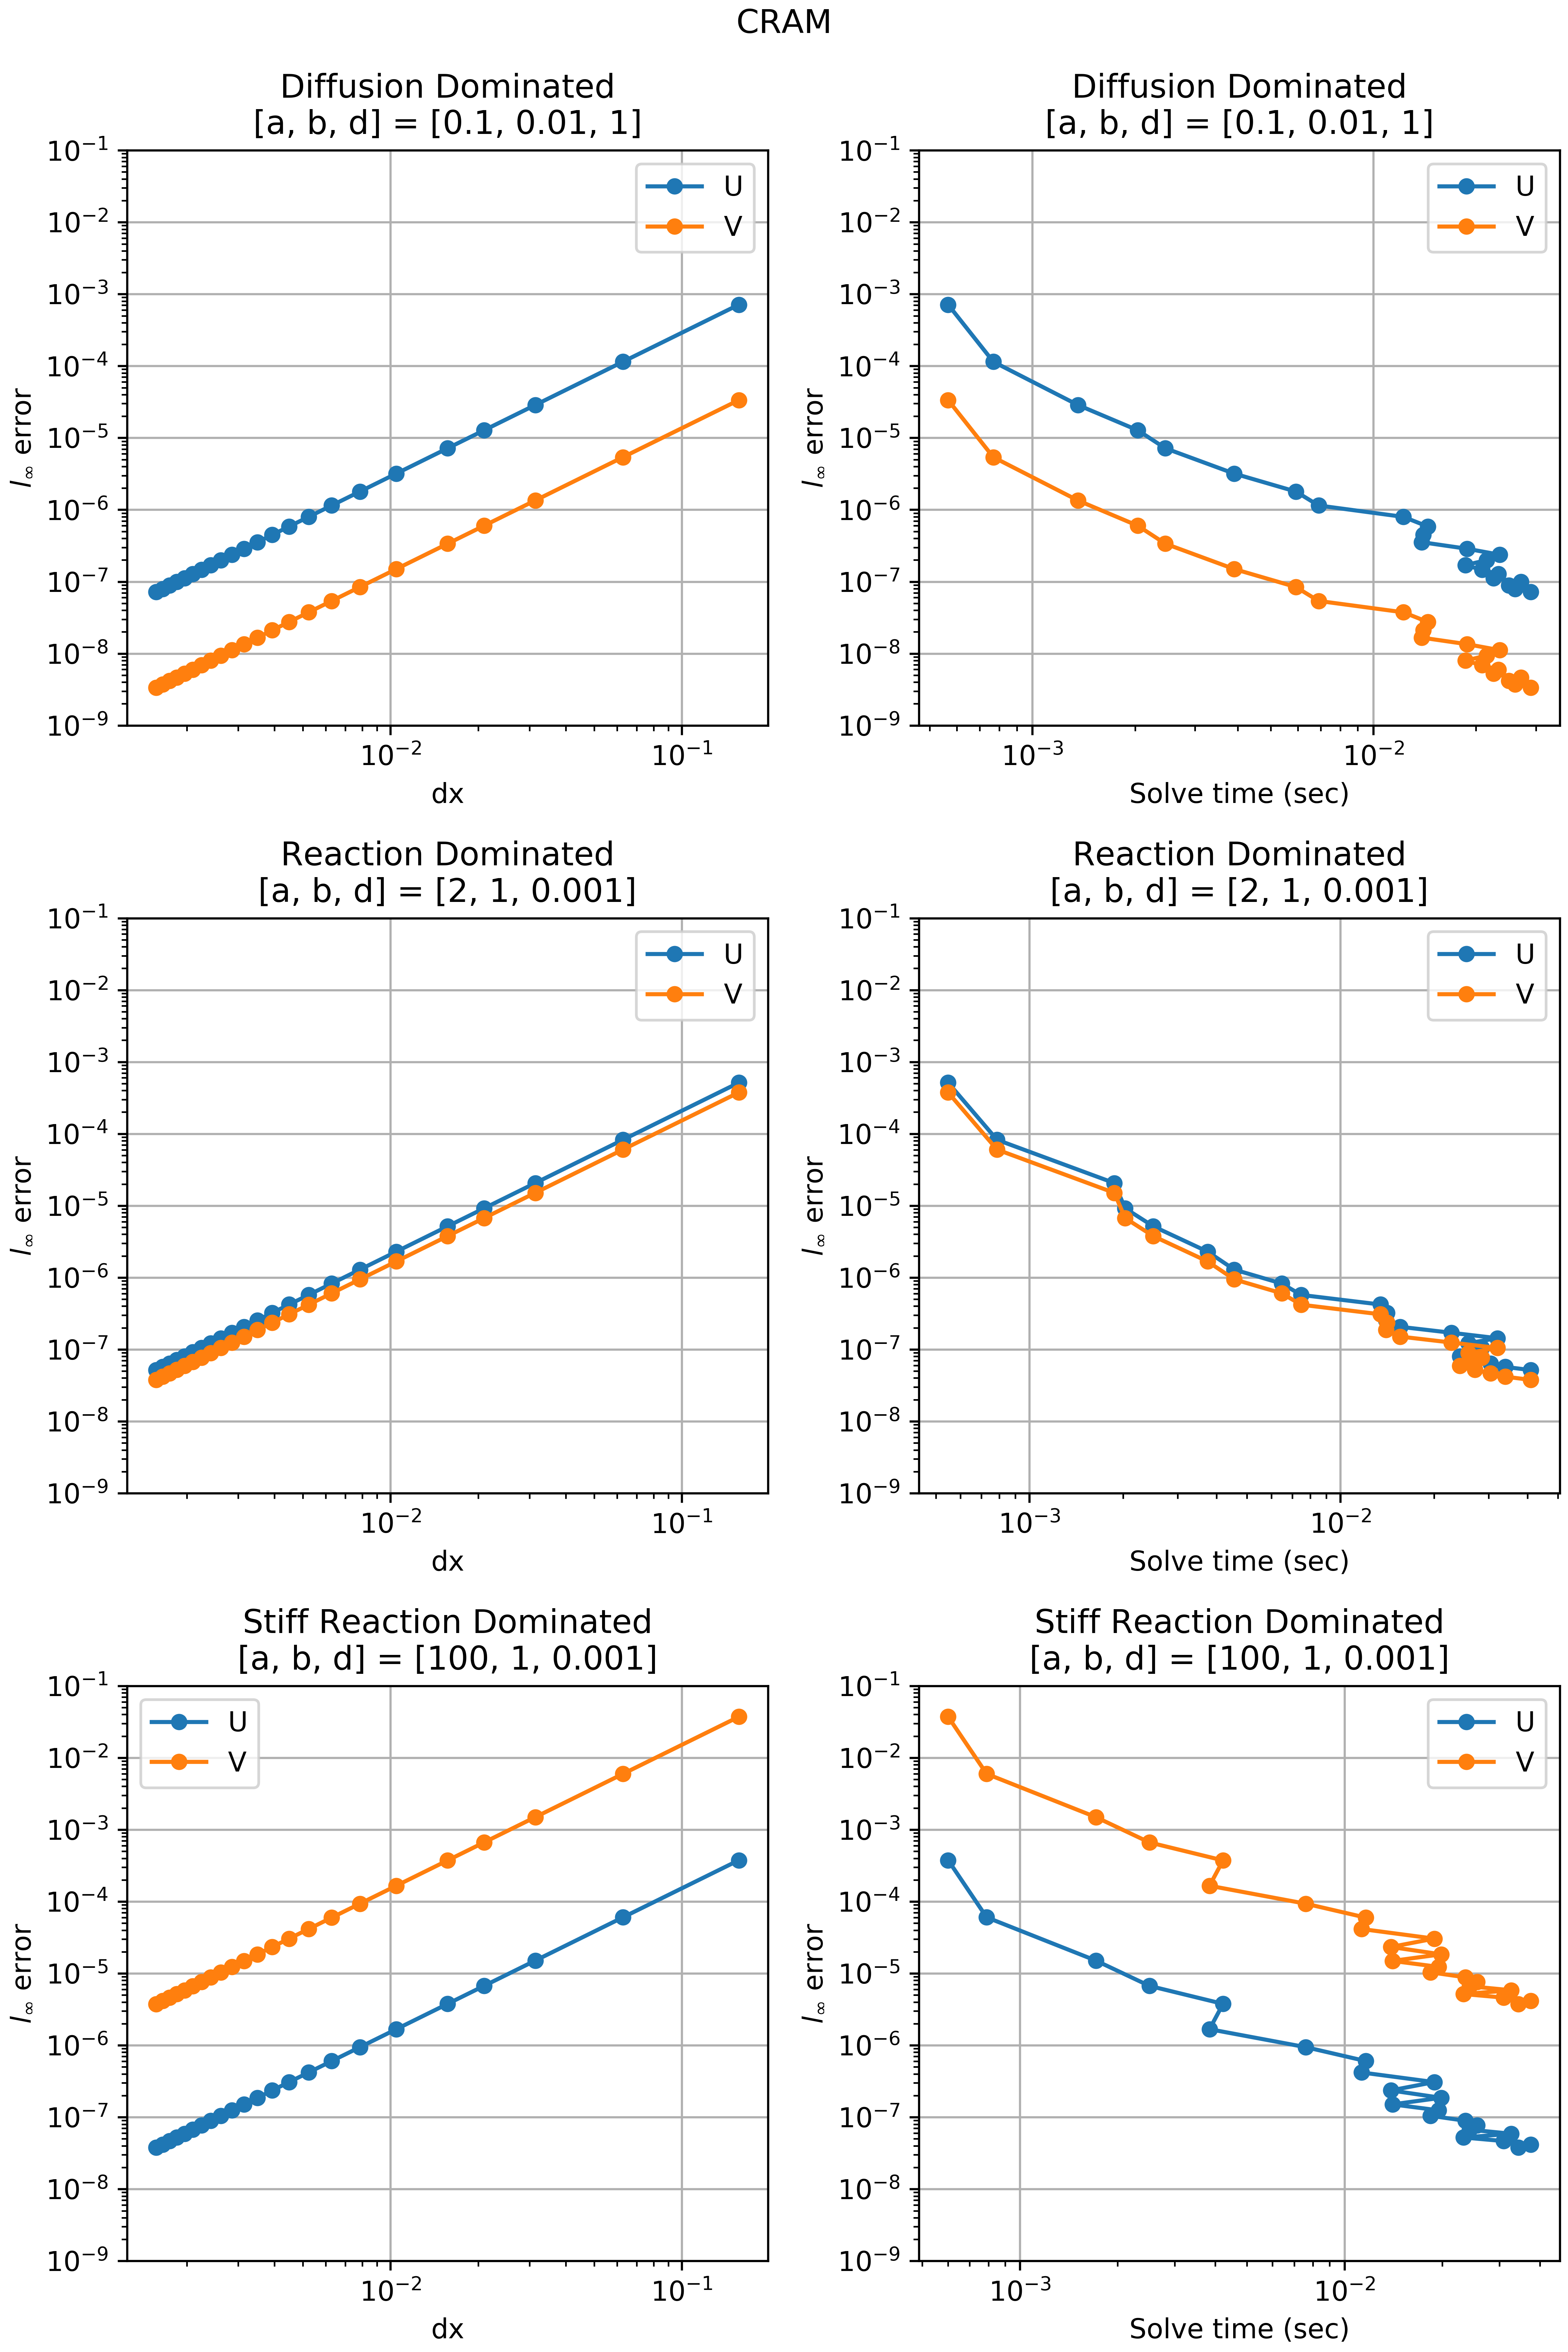
\includegraphics[width=5.75in]{images/CRAMproblem2.png}\\
  \caption{Error for Problem 2 Using CRAM}
  \label{fig:errorProblem2CRAM}
\end{figure} 


\begin{figure}[t]
  \centering
  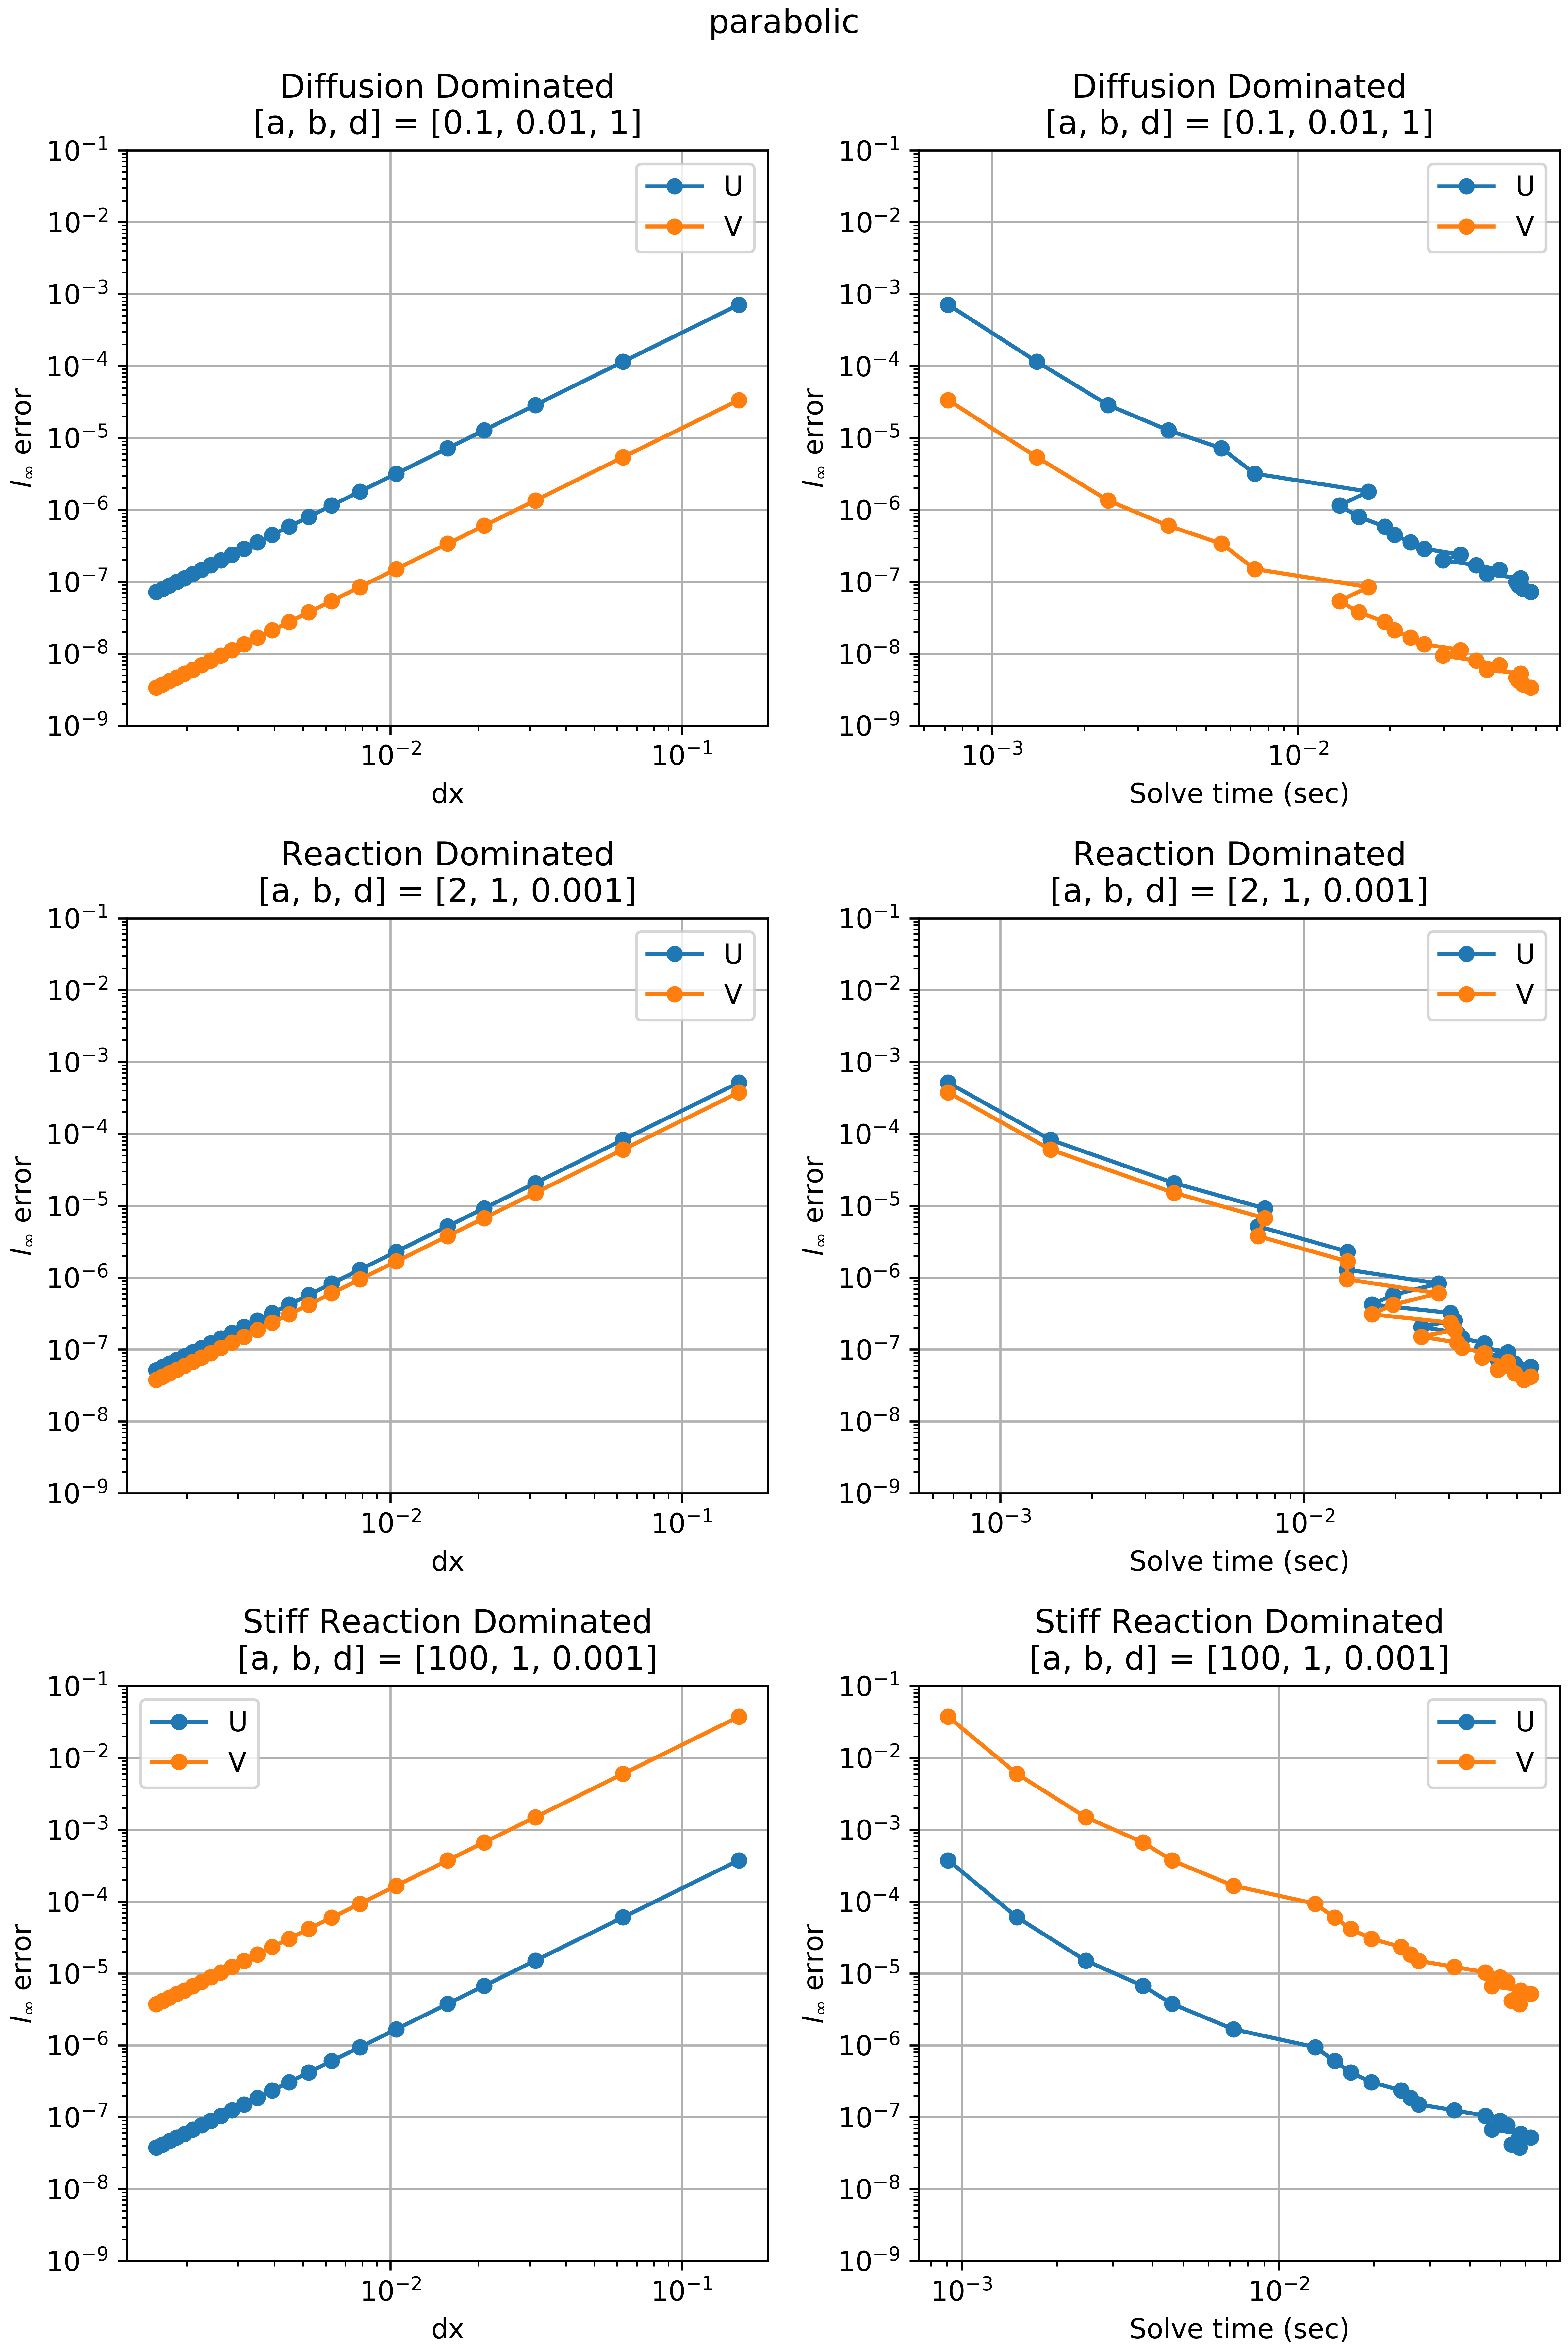
\includegraphics[width=5.75in]{images/parabolicproblem2.png}\\
  \caption{Error for Problem 2 Using Parabolic}
  \label{fig:errorProblem2parabolic}
\end{figure} 

\begin{figure}[t]
  \centering
  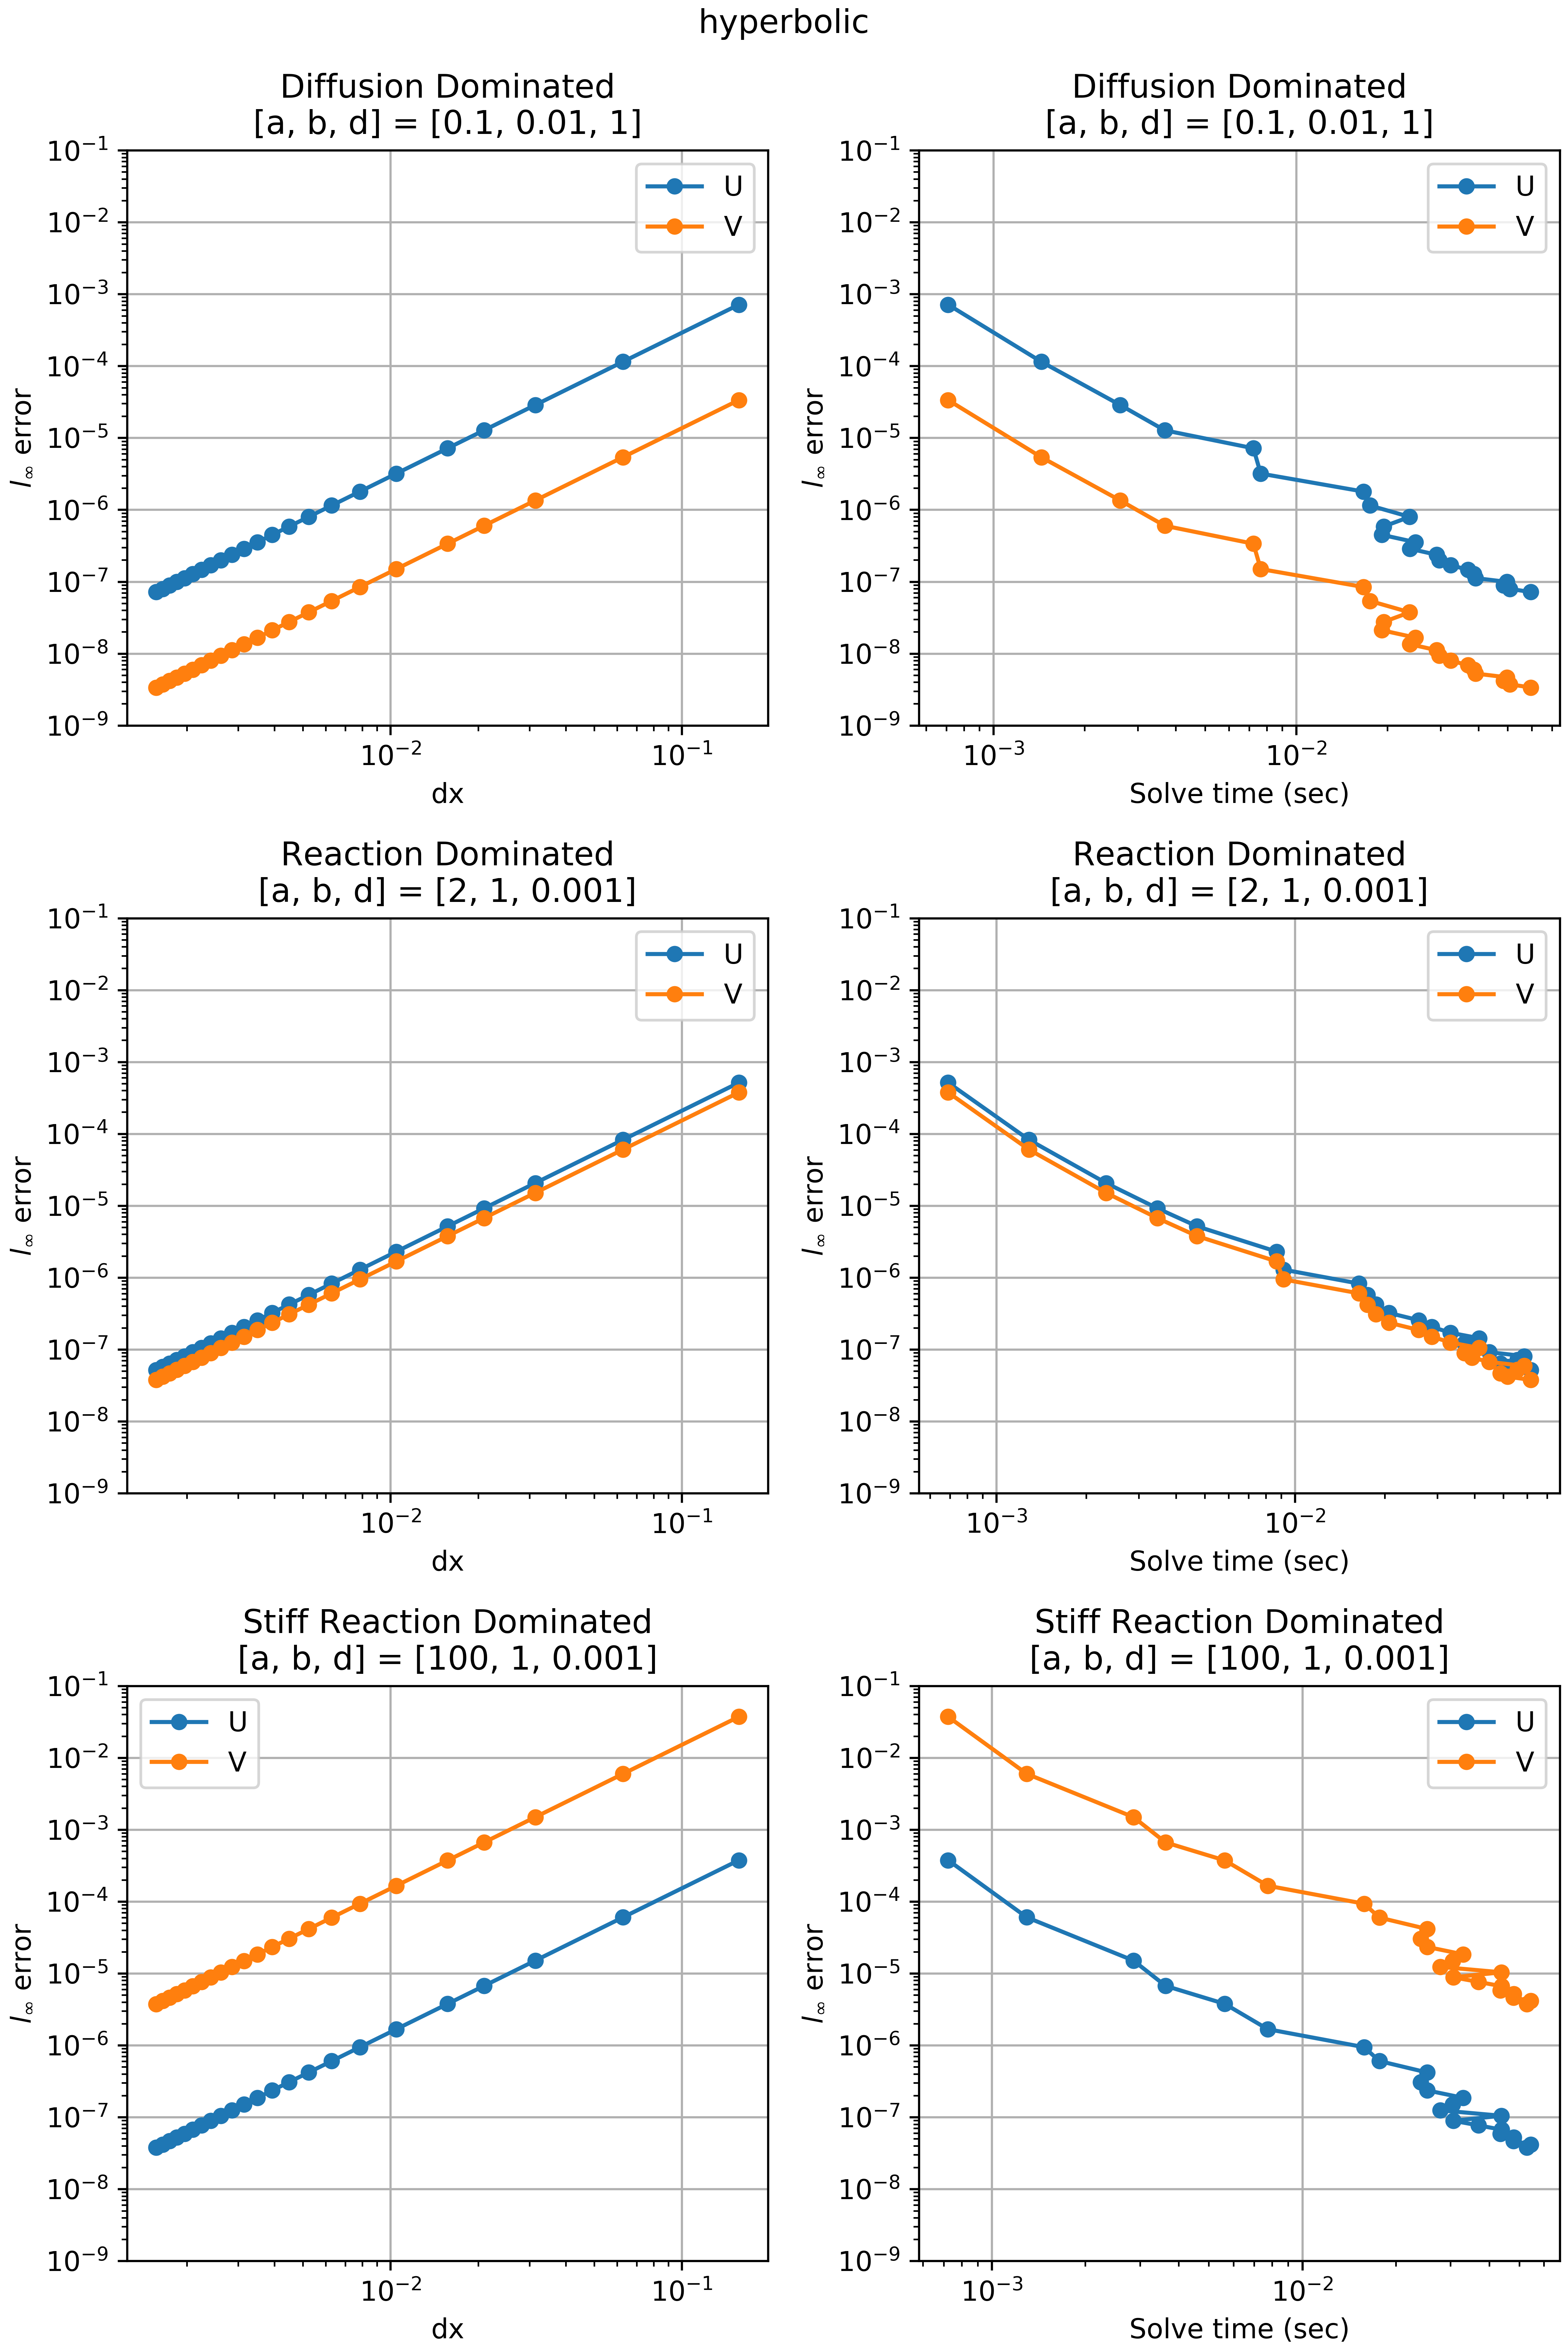
\includegraphics[width=5.75in]{images/hyperbolicproblem2.png}\\
  \caption{Error for Problem 2 Using Hyperbolic}
  \label{fig:errorProblem2hyperbolic}
\end{figure} 

\begin{figure}[t]
  \centering
  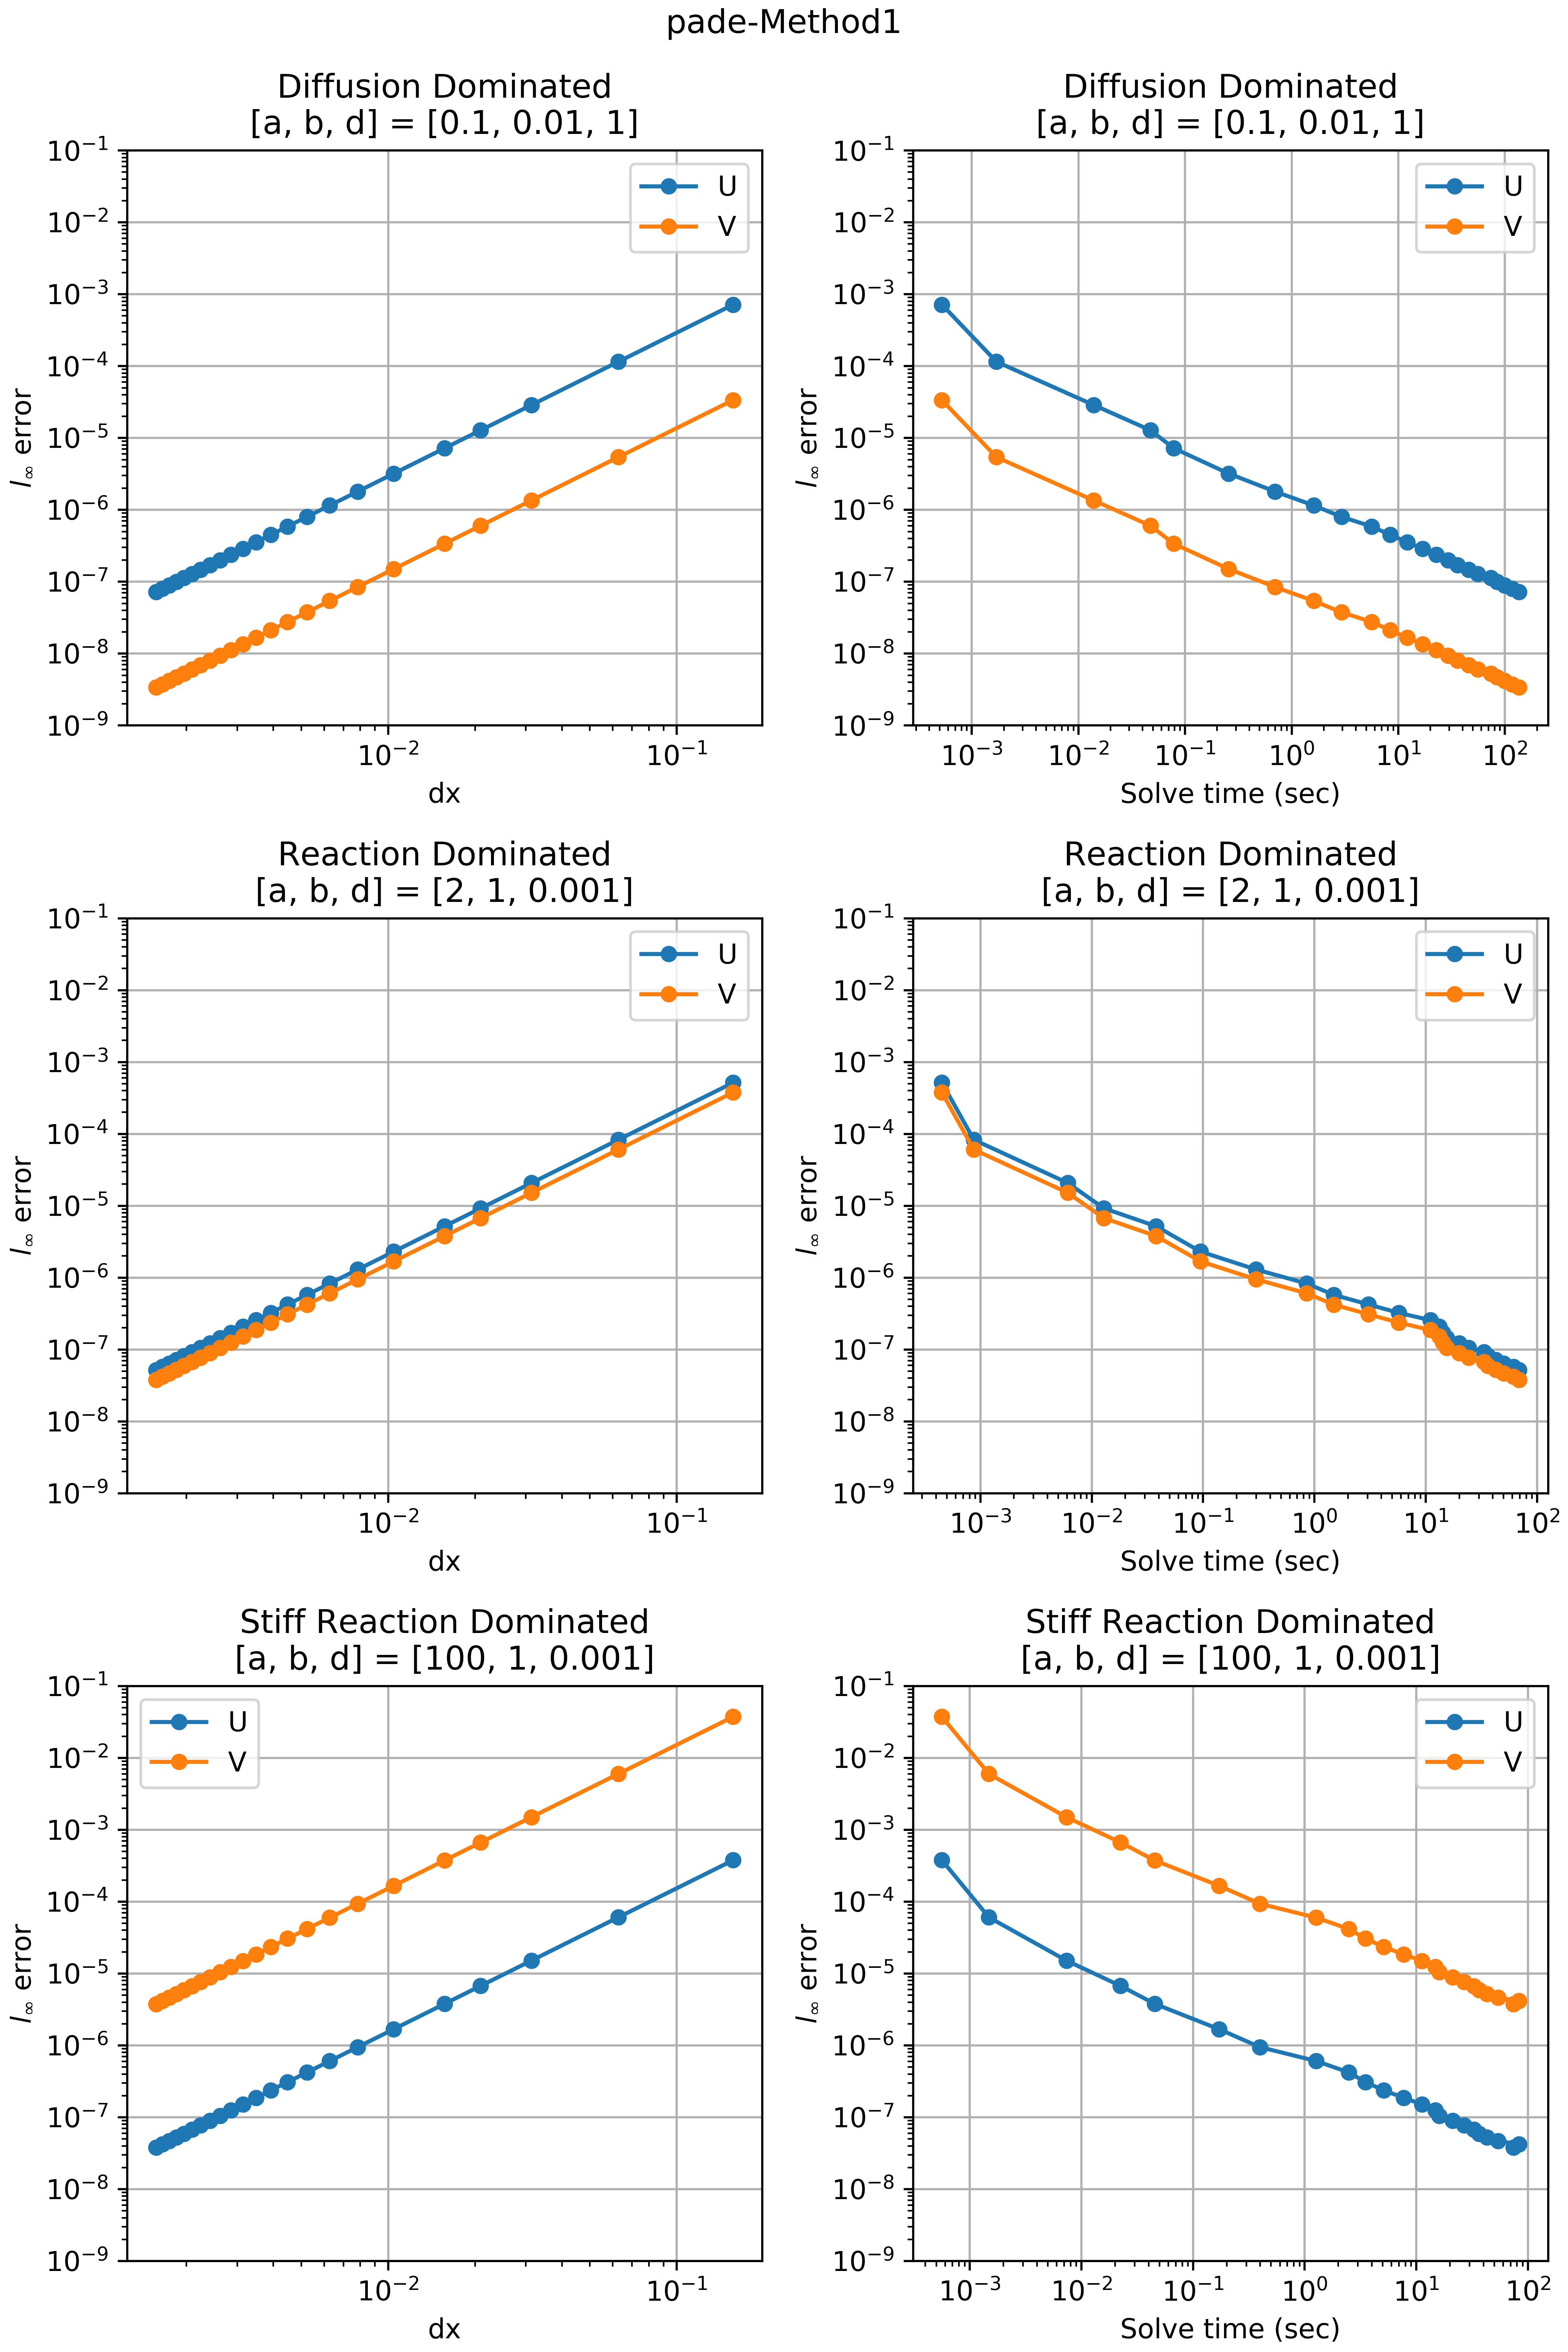
\includegraphics[width=5.75in]{images/pade-Method1problem2.png}\\
  \caption{Error for Problem 2 Using Pade-Method1}
  \label{fig:errorProblem2padeM1}
\end{figure} 

\begin{figure}[t]
  \centering
  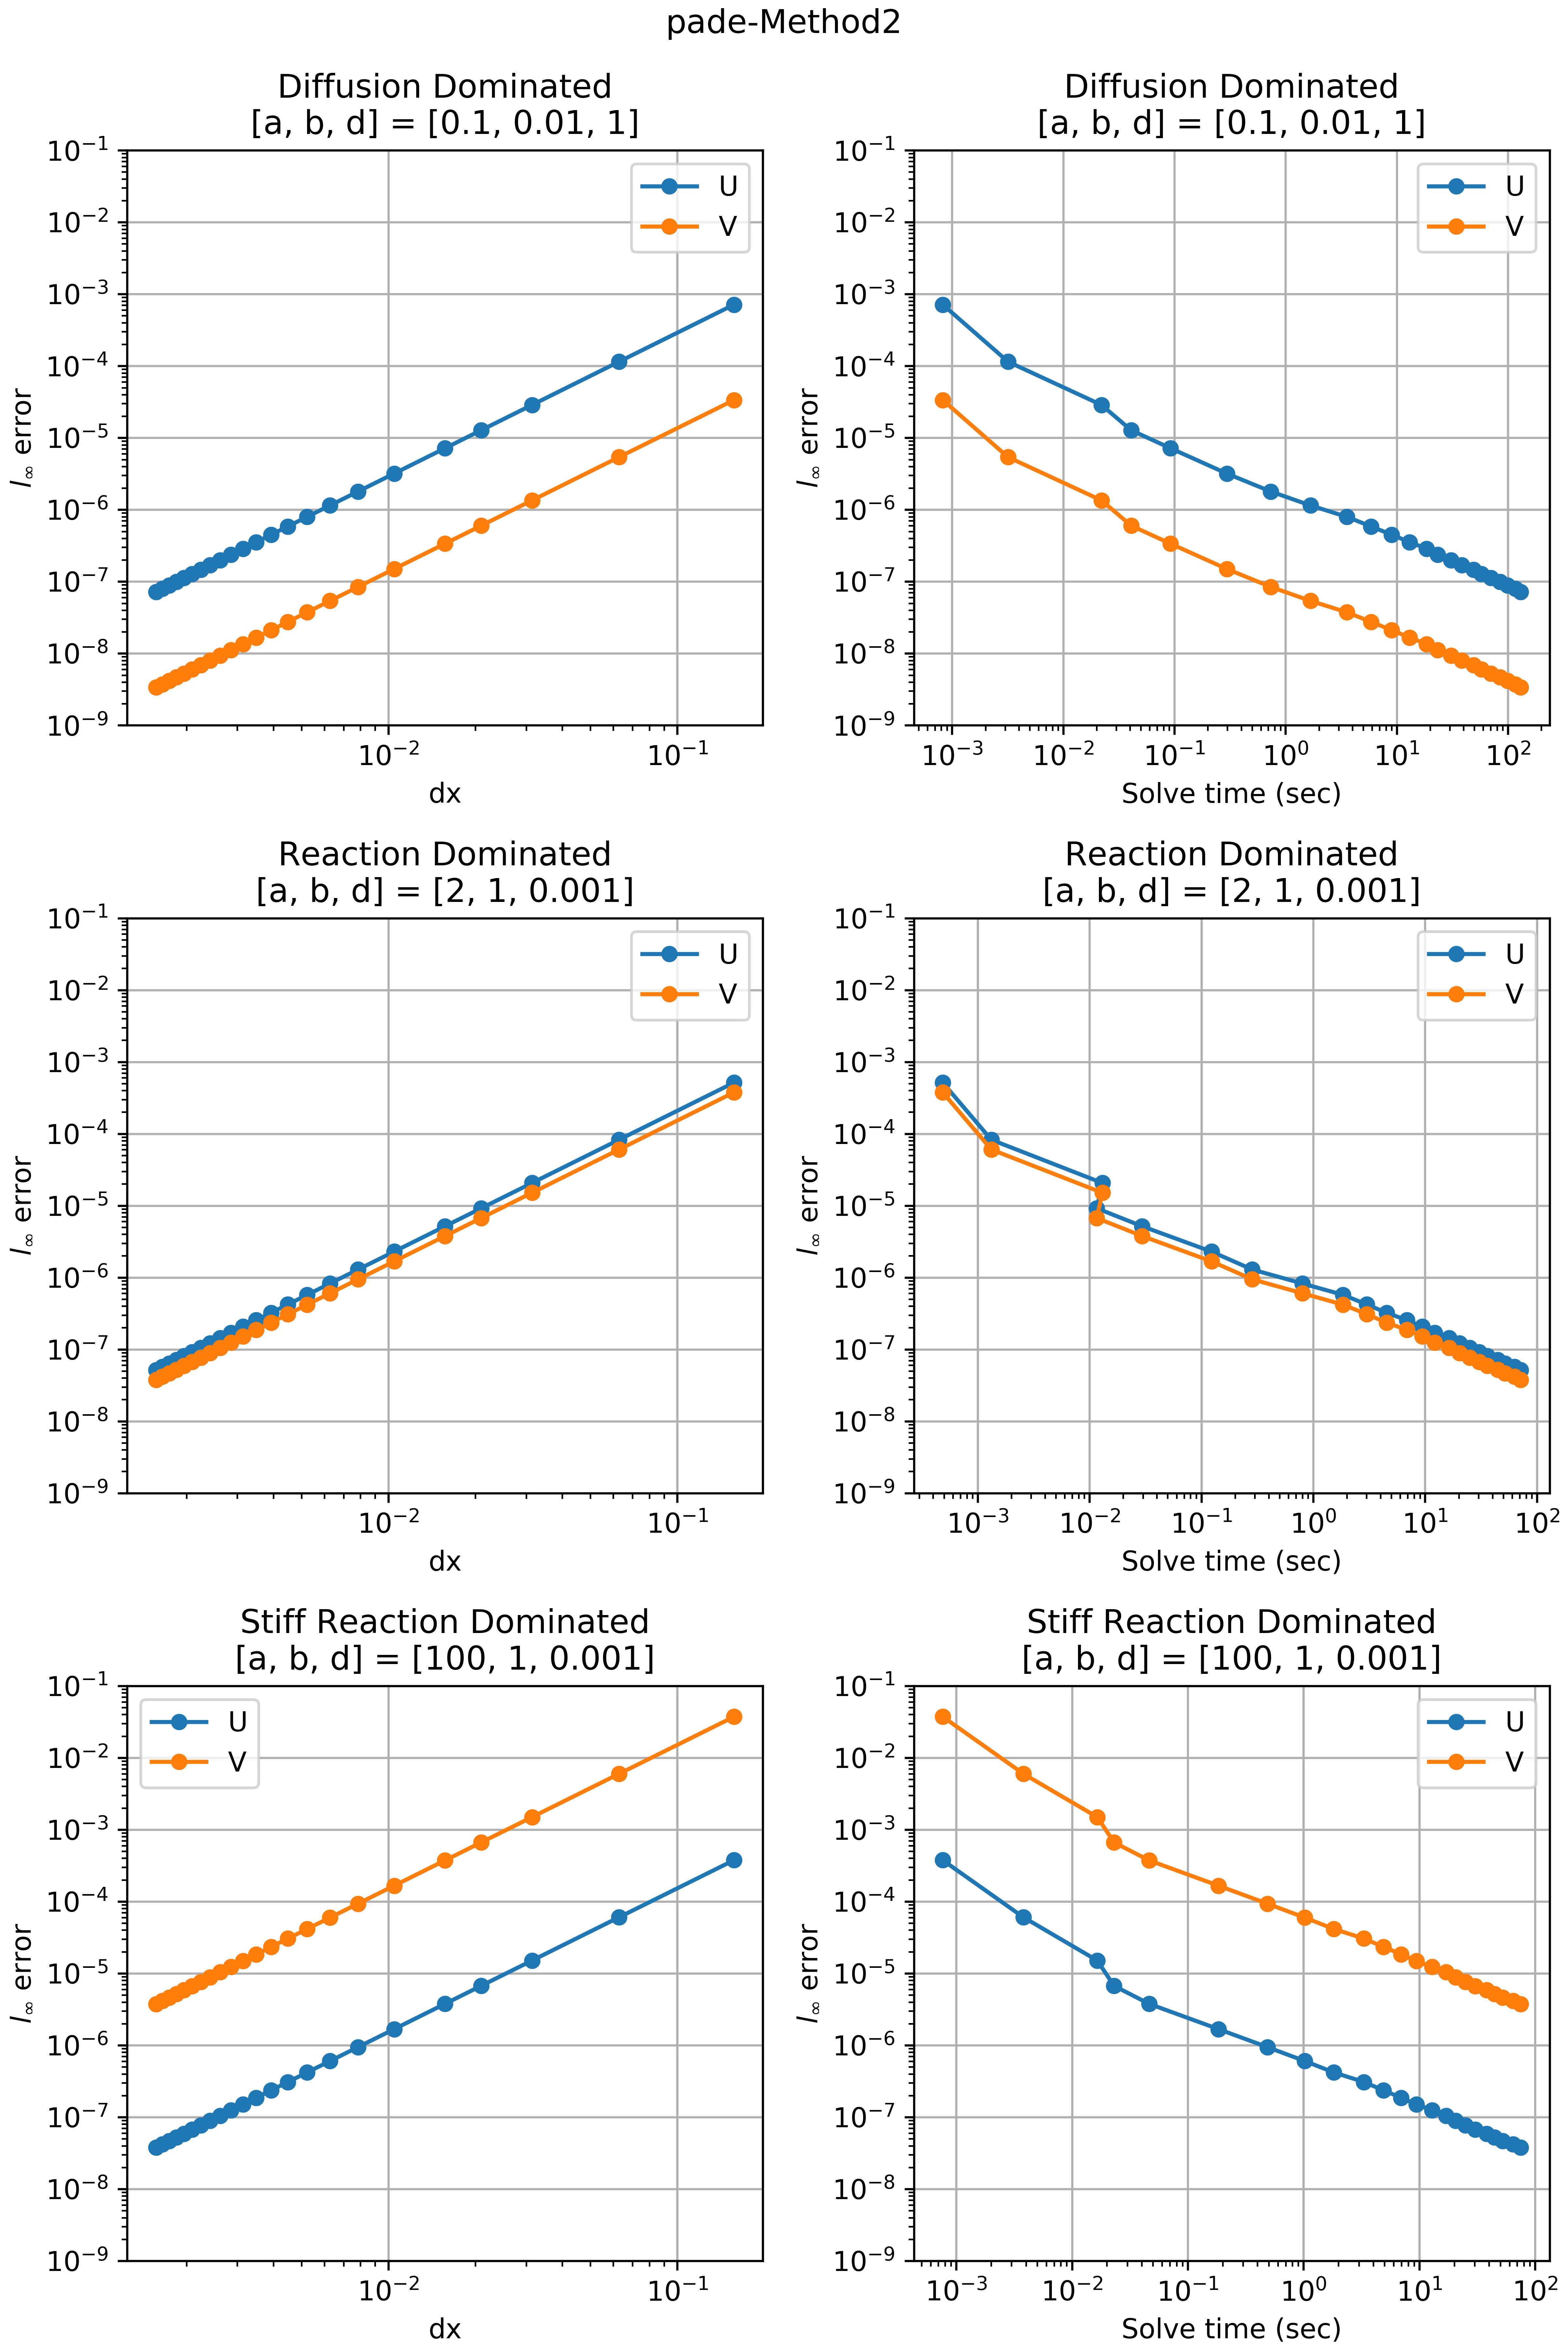
\includegraphics[width=5.75in]{images/pade-Method2problem2.png}\\
  \caption{Error for Problem 2 Using Pade-Method2}
  \label{fig:errorProblem2padeM2}
\end{figure} 

\begin{figure}[t]
  \centering
  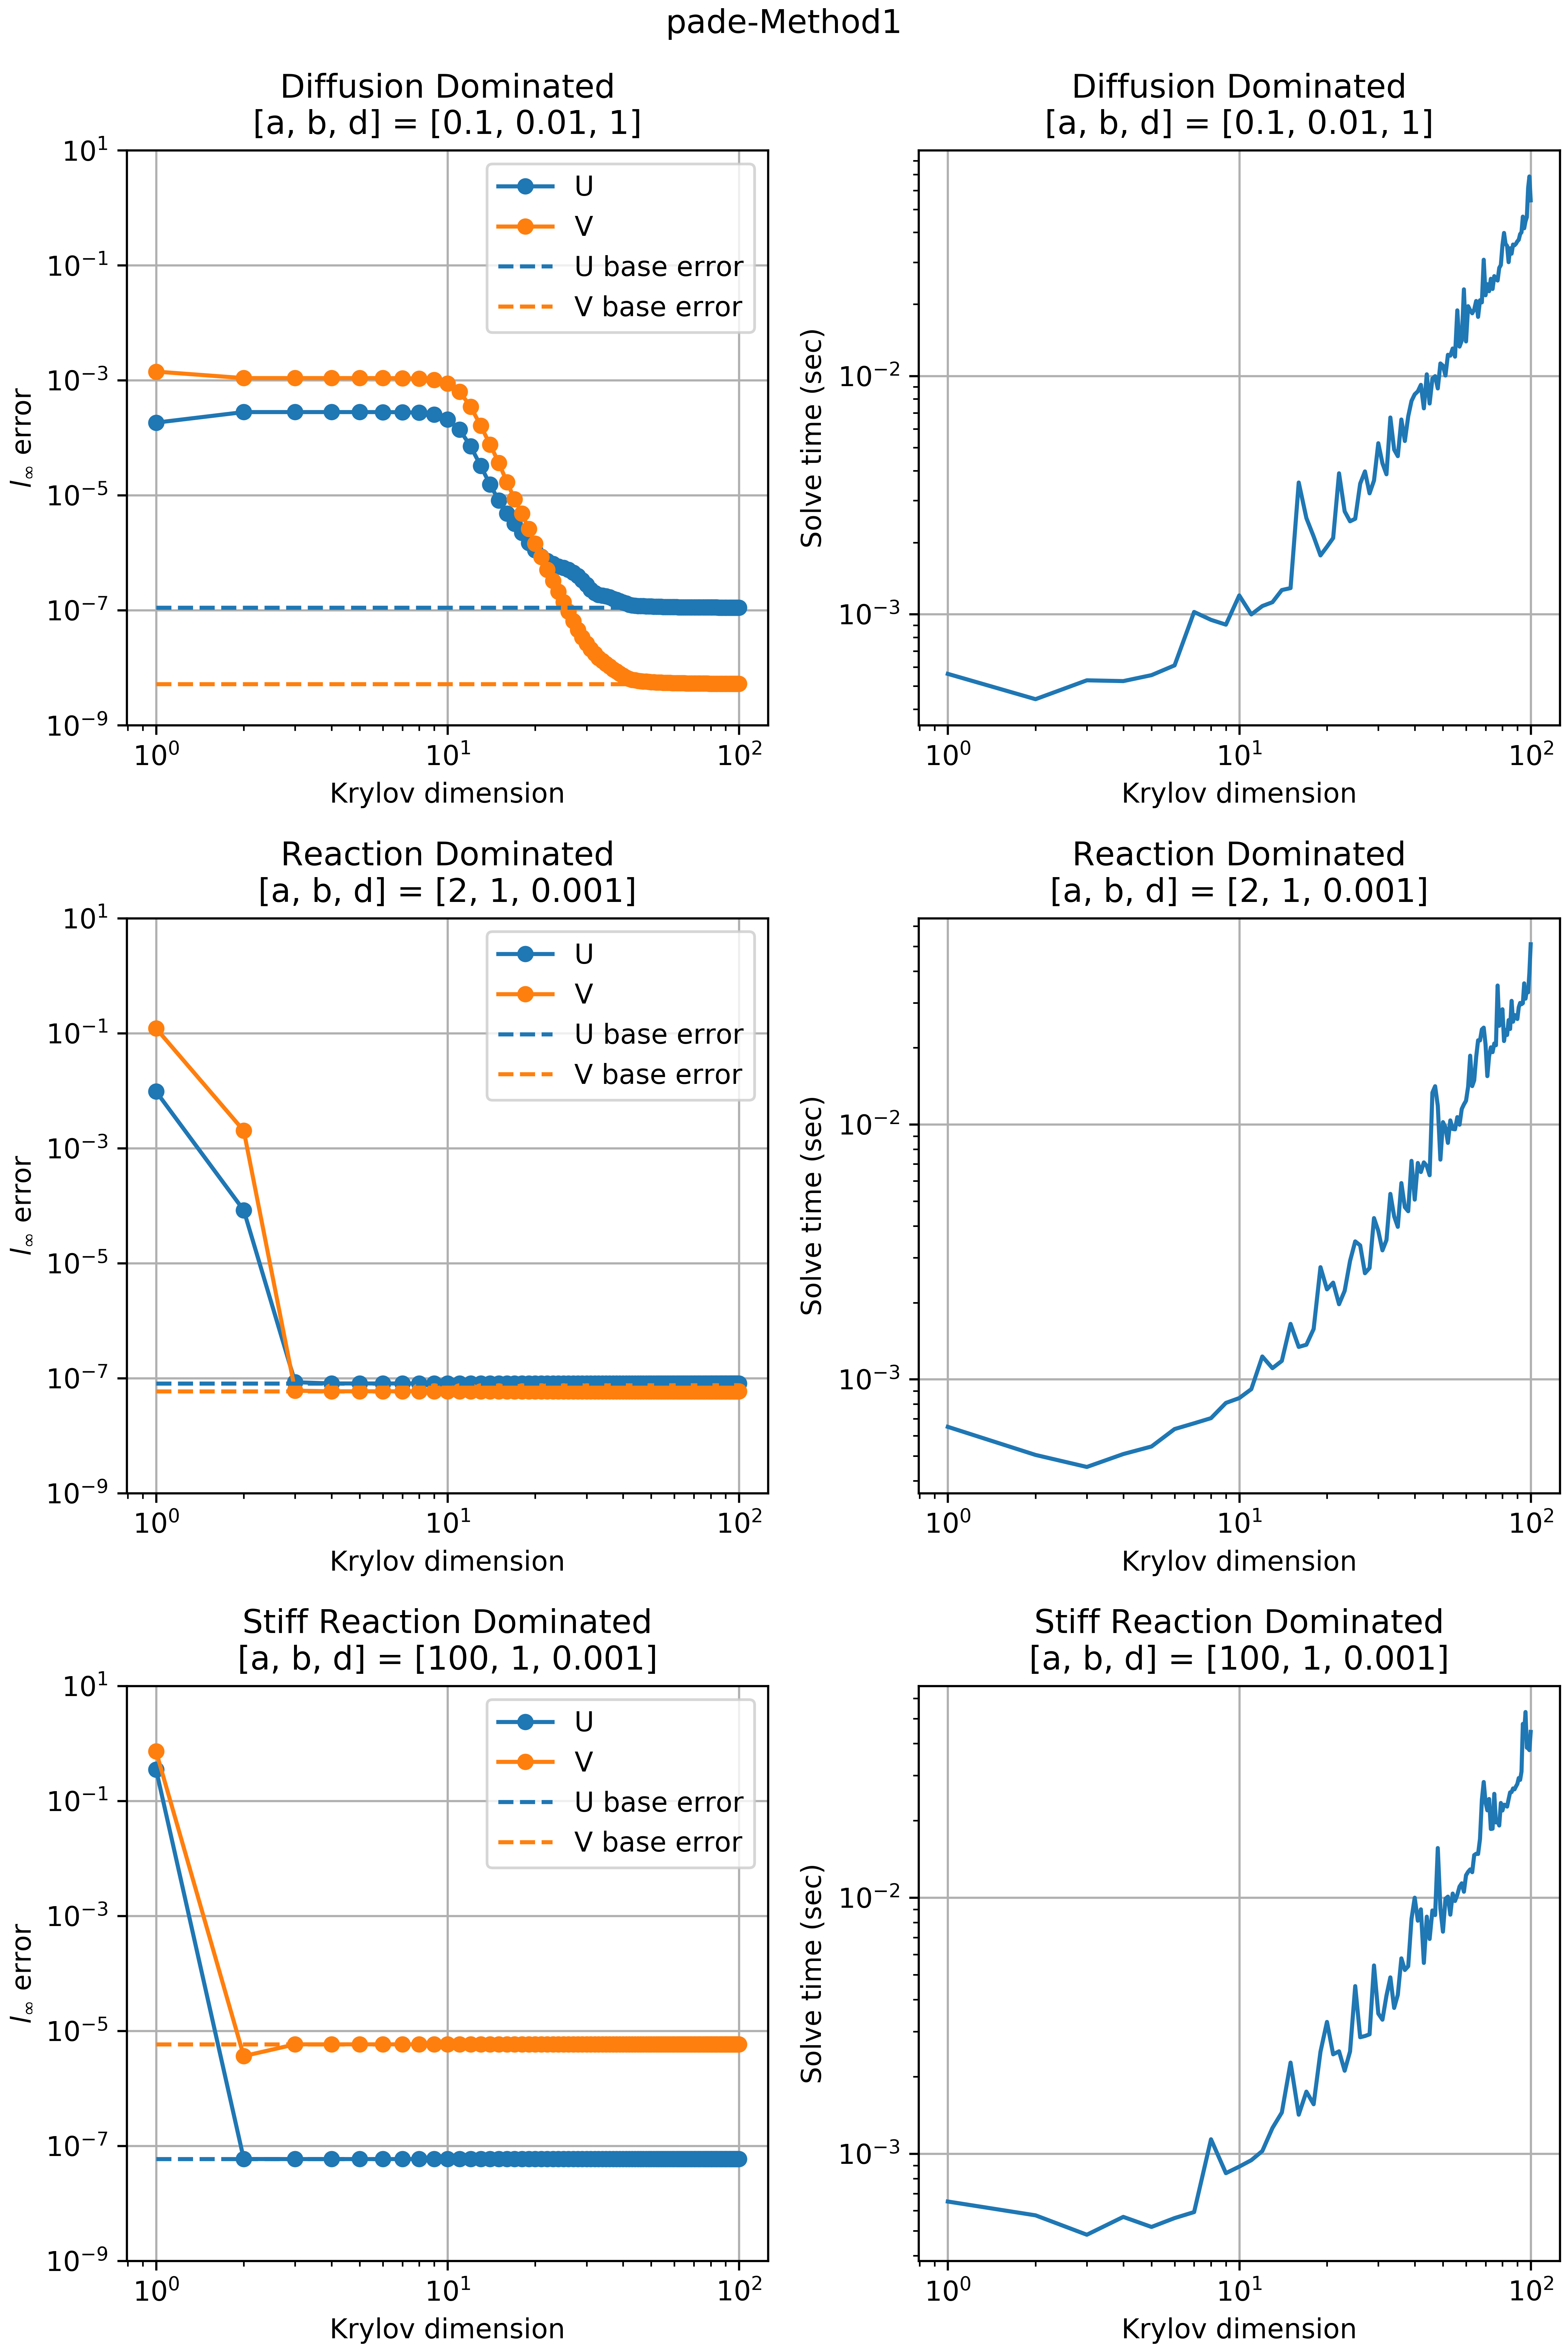
\includegraphics[width=5.75in]{images/pade-Method1KrylovProblem2.png}\\
  \caption{Krylov Approximation for Problem 2 Using Pade-Method1}
  \label{fig:errorProblem2padeM1Krylov}
\end{figure} 

\begin{figure}[t]
  \centering
  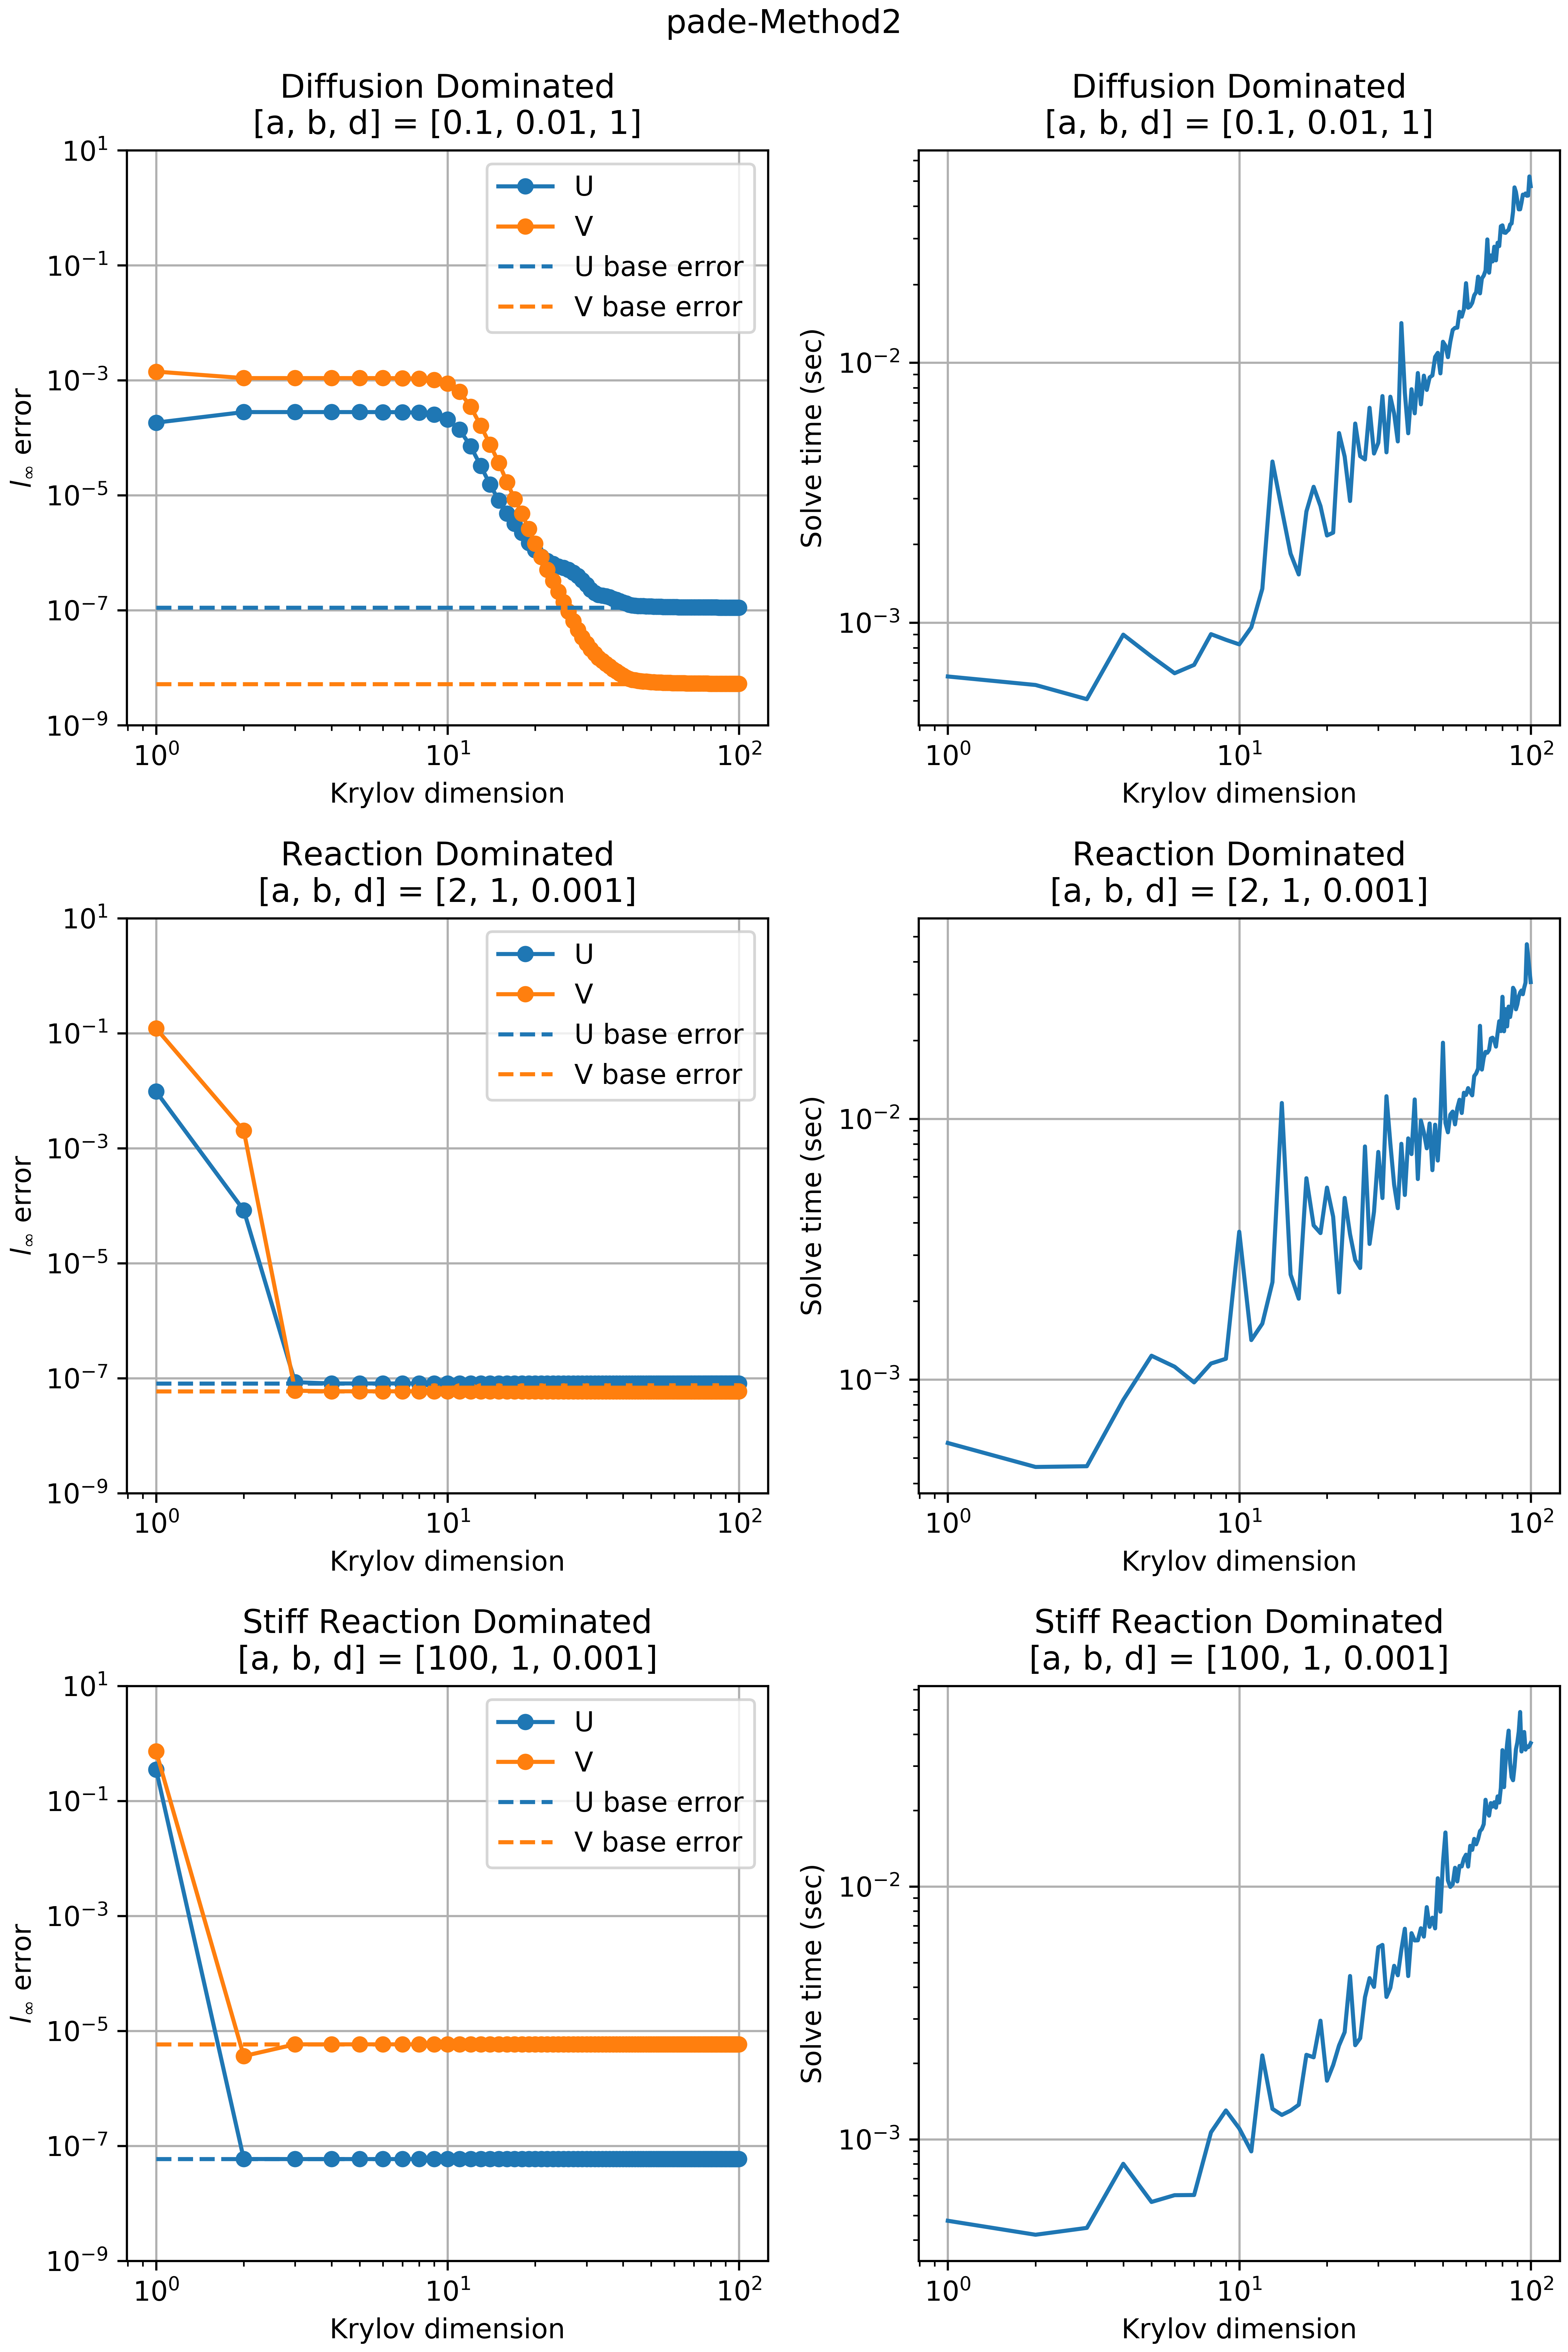
\includegraphics[width=5.75in]{images/pade-Method2KrylovProblem2.png}\\
  \caption{Krylov Approximation for Problem 2 Using Pade-Method2}
  \label{fig:errorProblem2padeM2Krylov}
\end{figure} 

\begin{figure}[t]
  \centering
  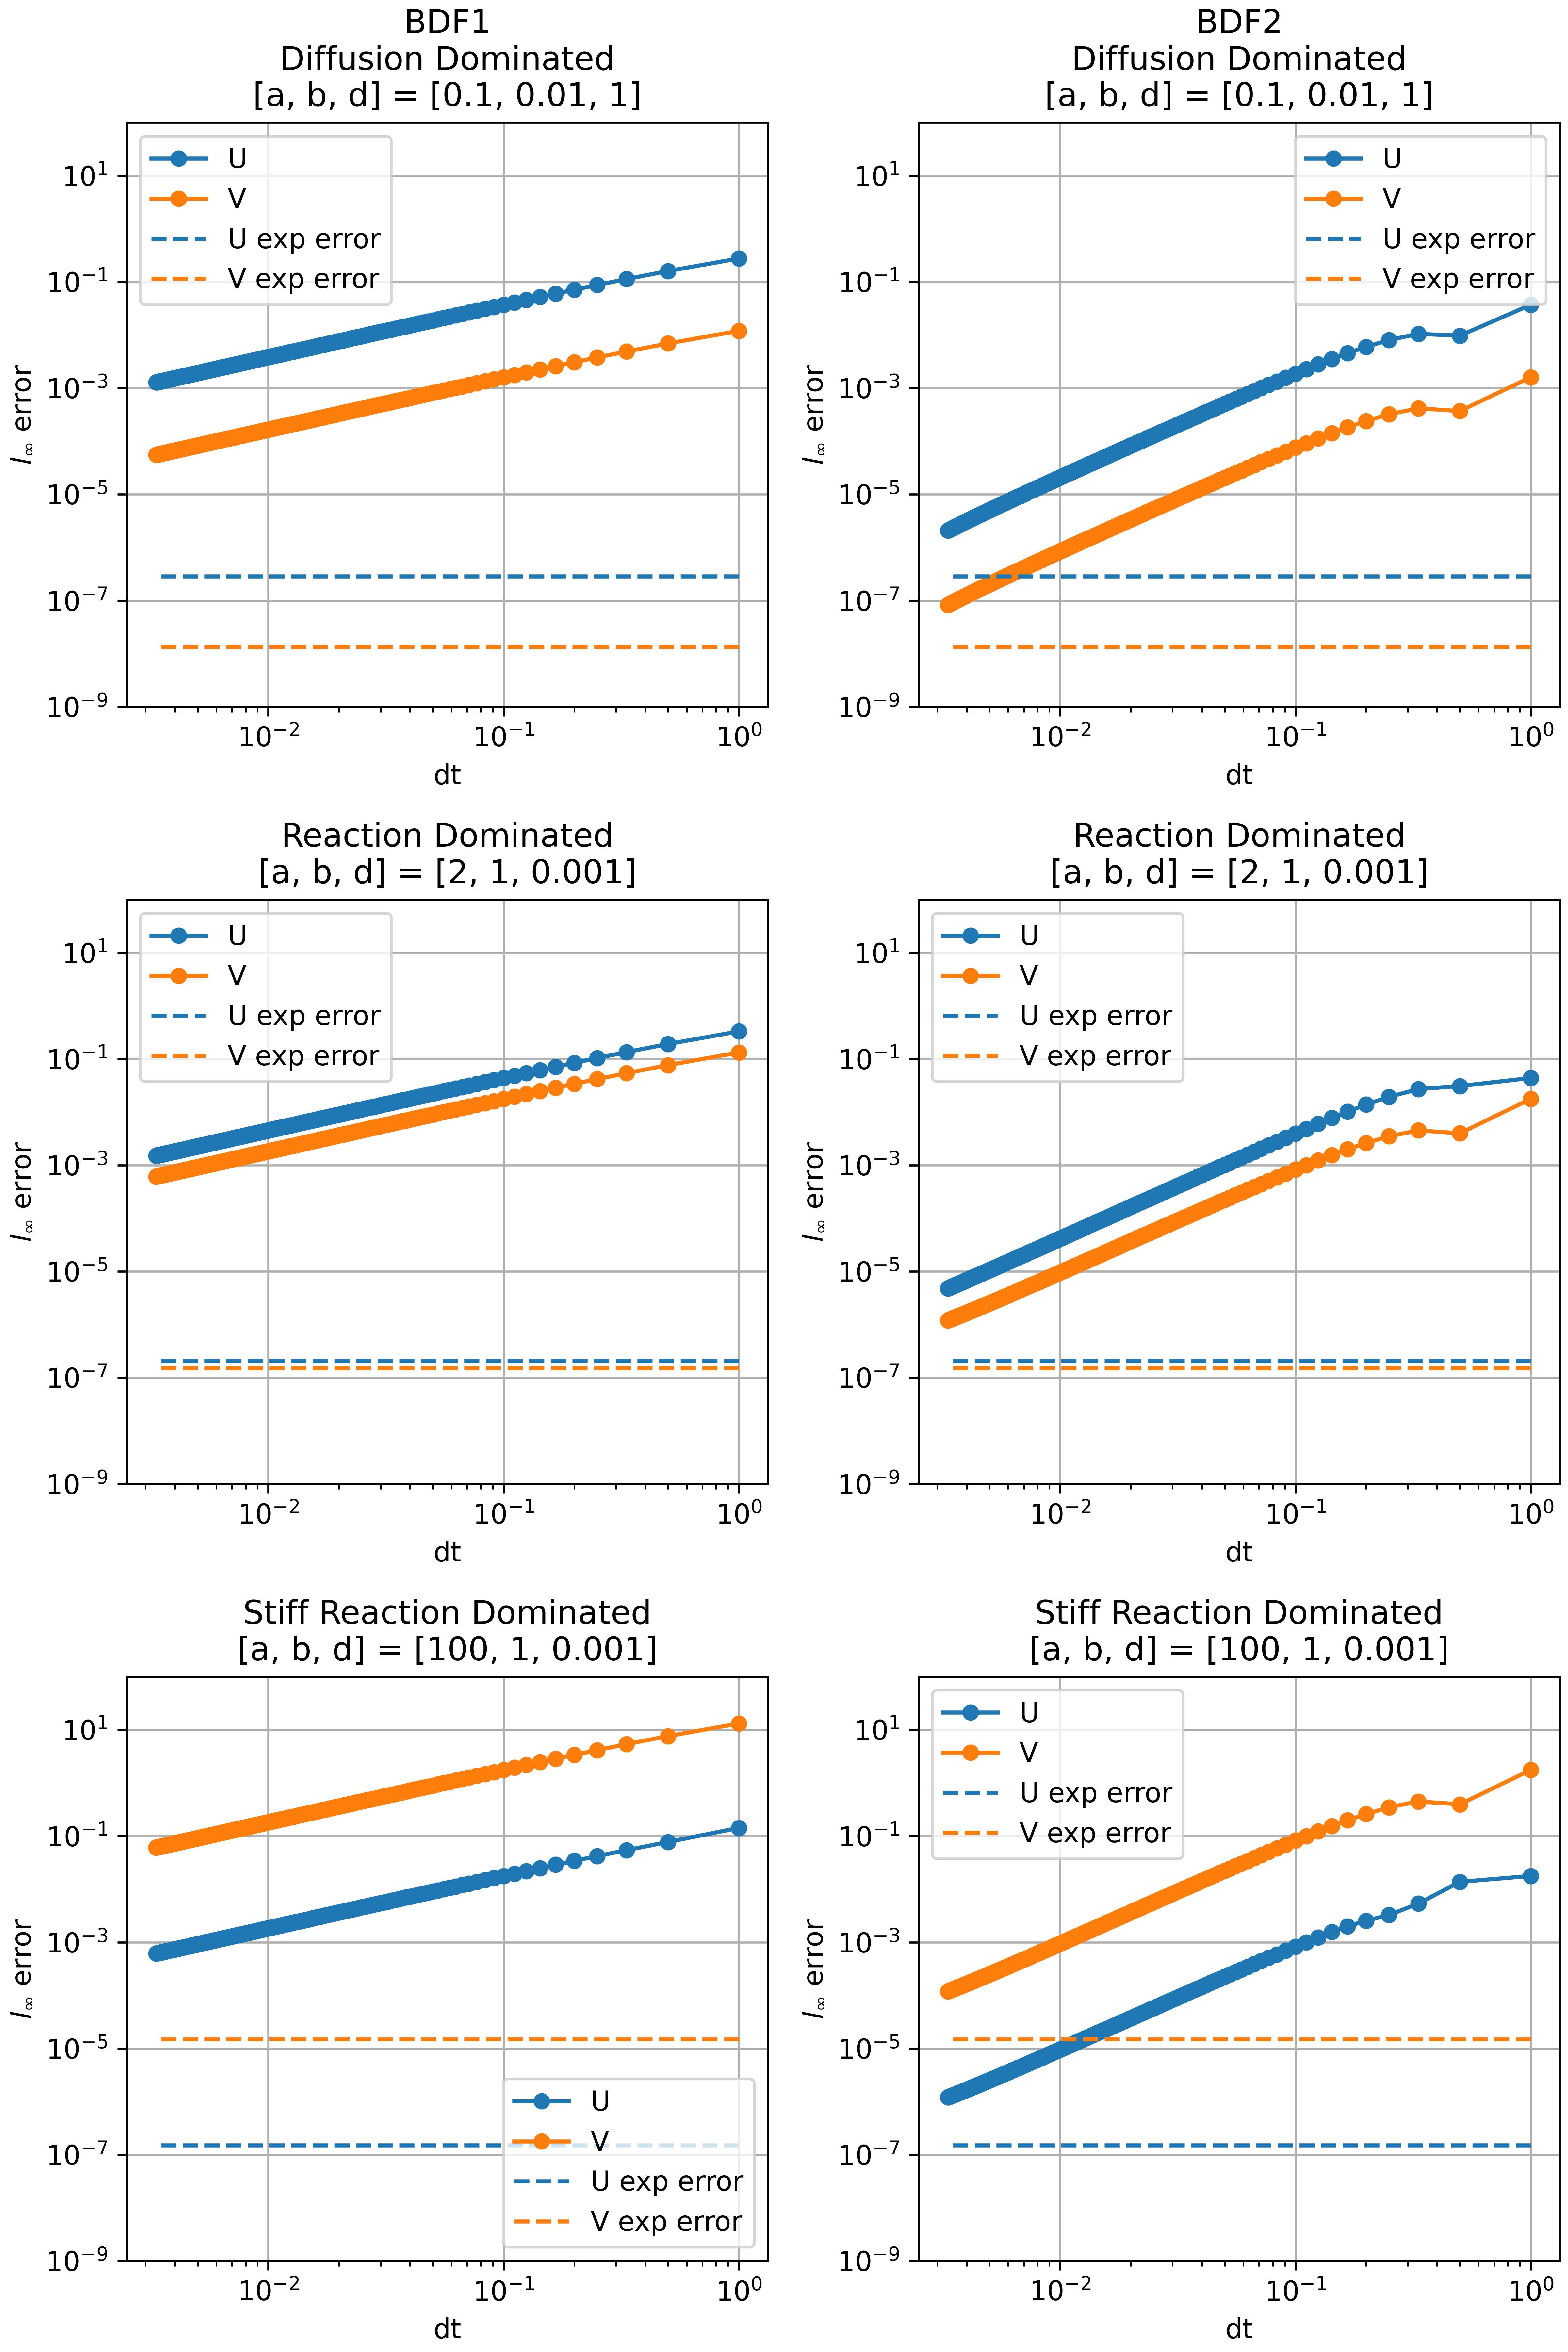
\includegraphics[width=5.75in]{images/BDF1BDF2problem2.png}\\
  \caption{BDF Solution for Problem 2 for Orders 1 and 2}
  \label{fig:errorProblem2BDF1and2}
\end{figure} 

\begin{figure}[t]
  \centering
  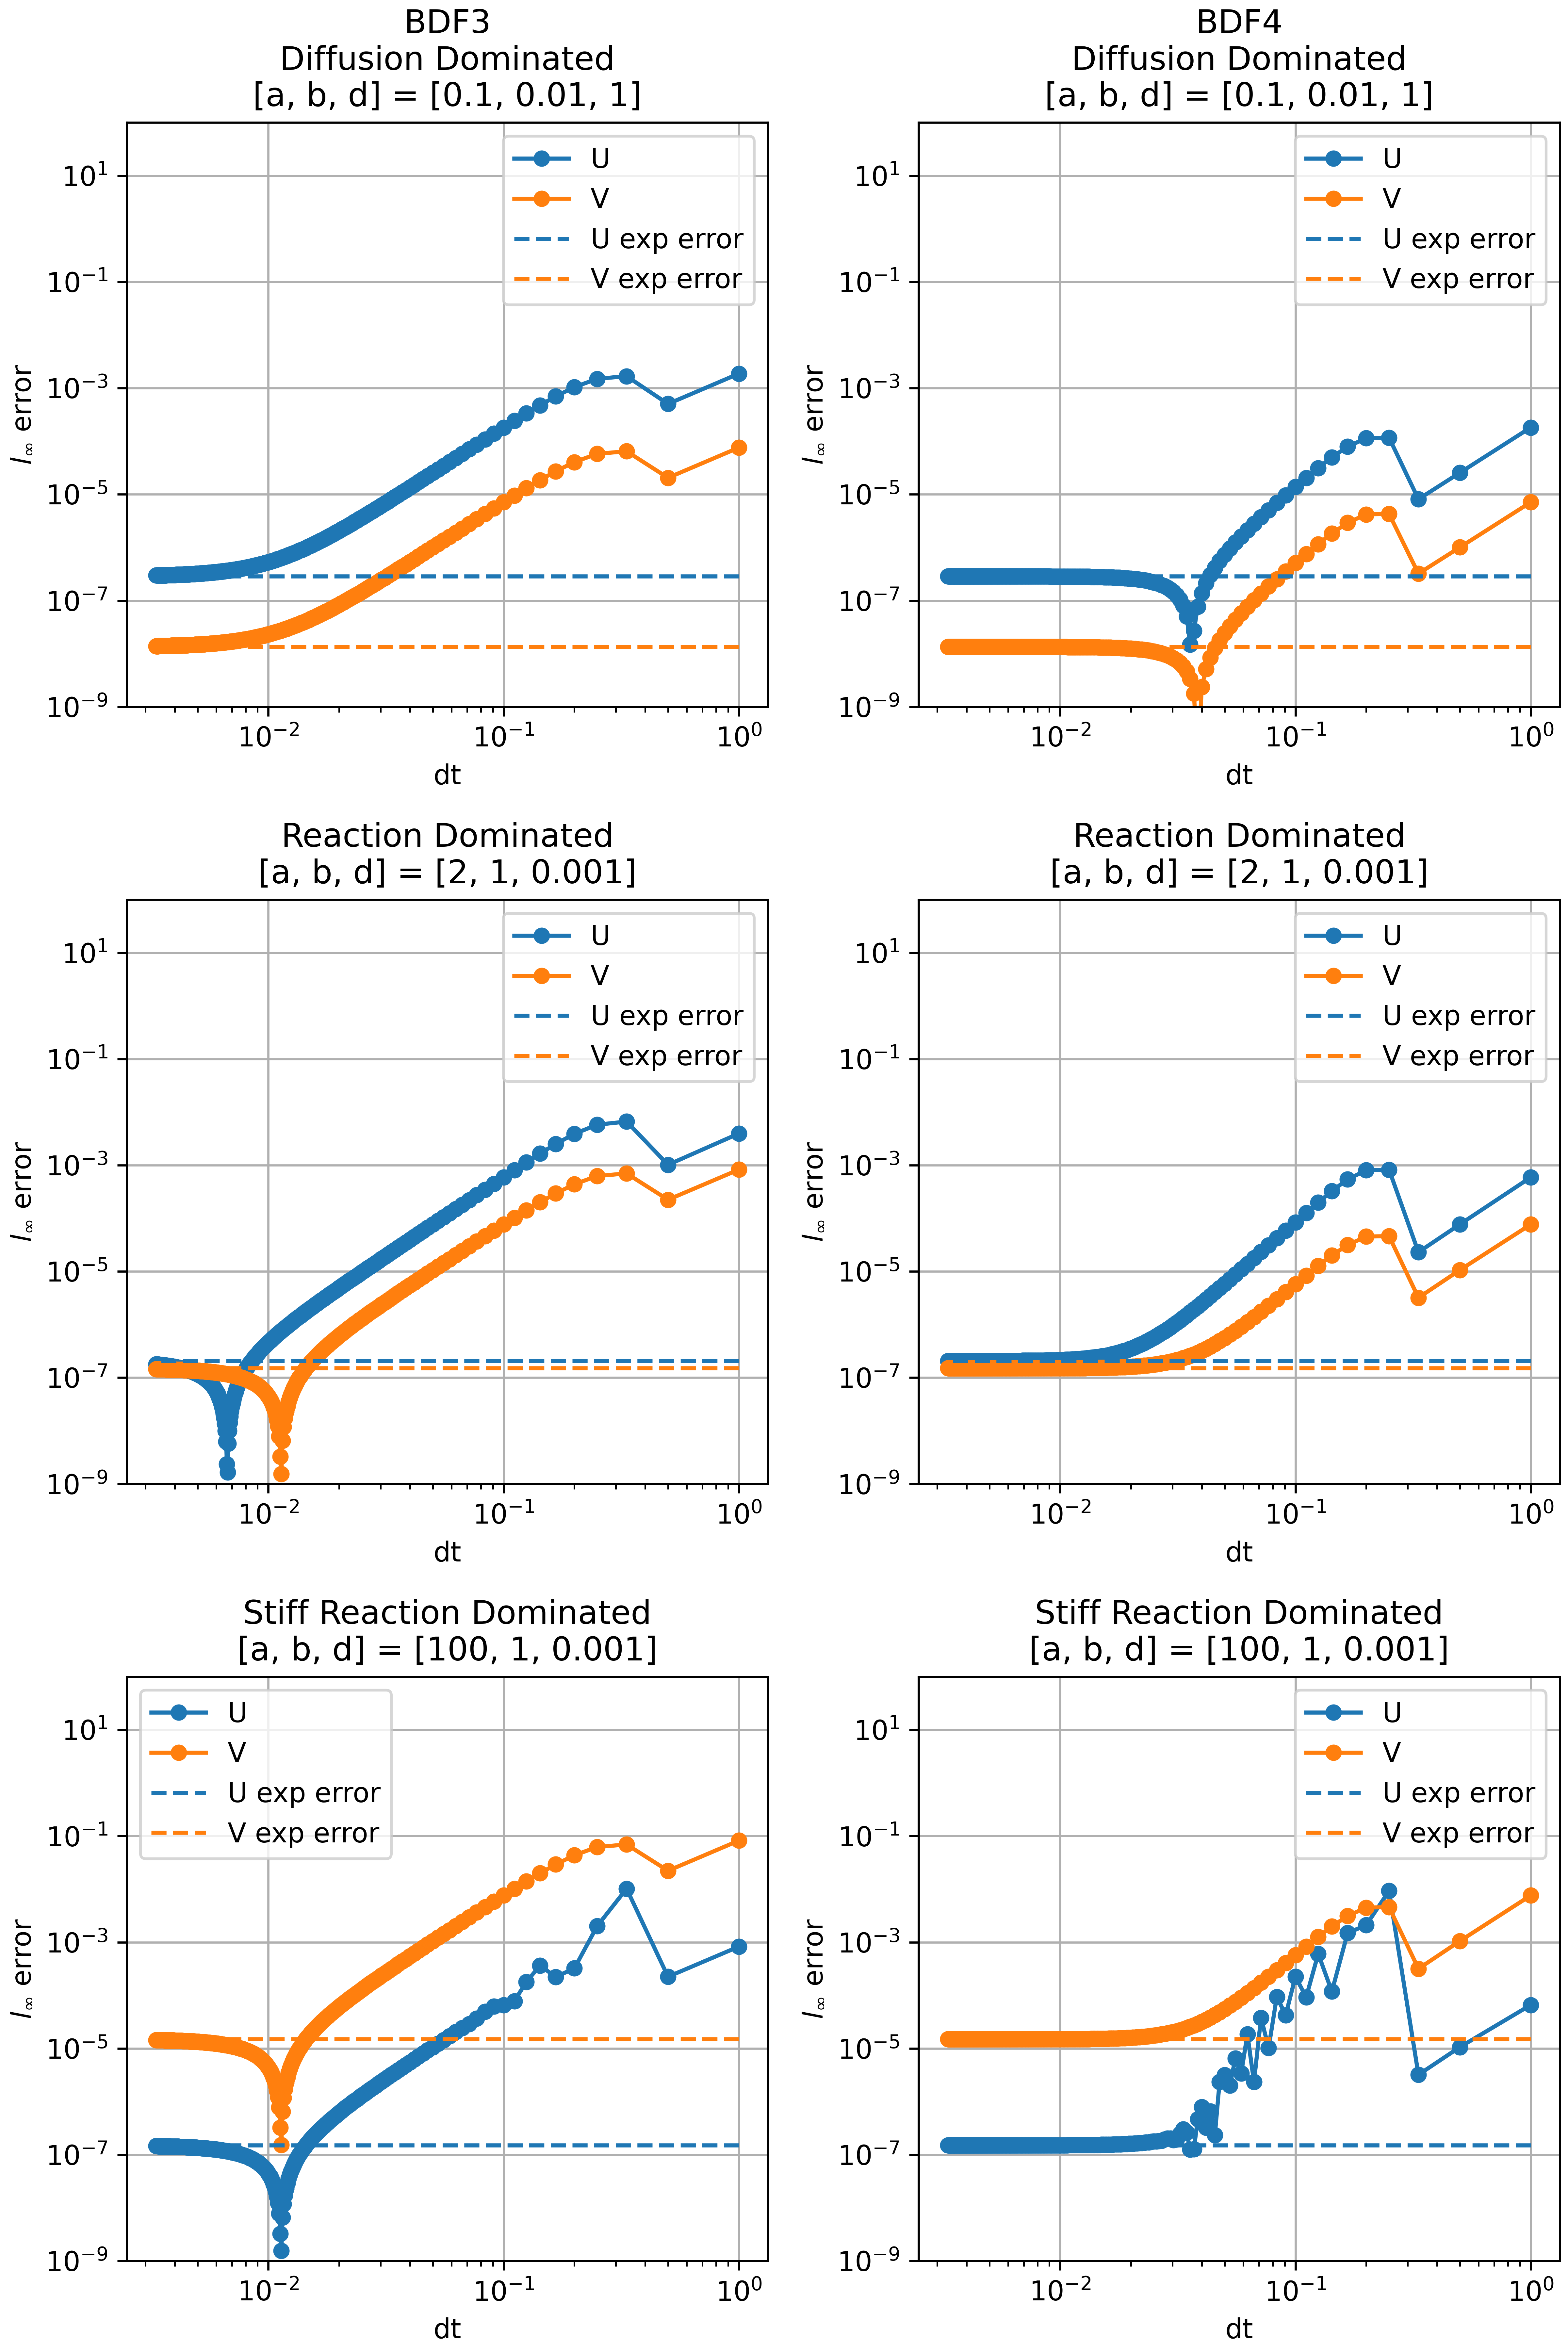
\includegraphics[width=5.75in]{images/BDF3BDF4problem2.png}\\
  \caption{BDF Solution for Problem 2 for Orders 3 and 4}
  \label{fig:errorProblem2BDF3and4}
\end{figure} 

\begin{figure}[t]
  \centering
  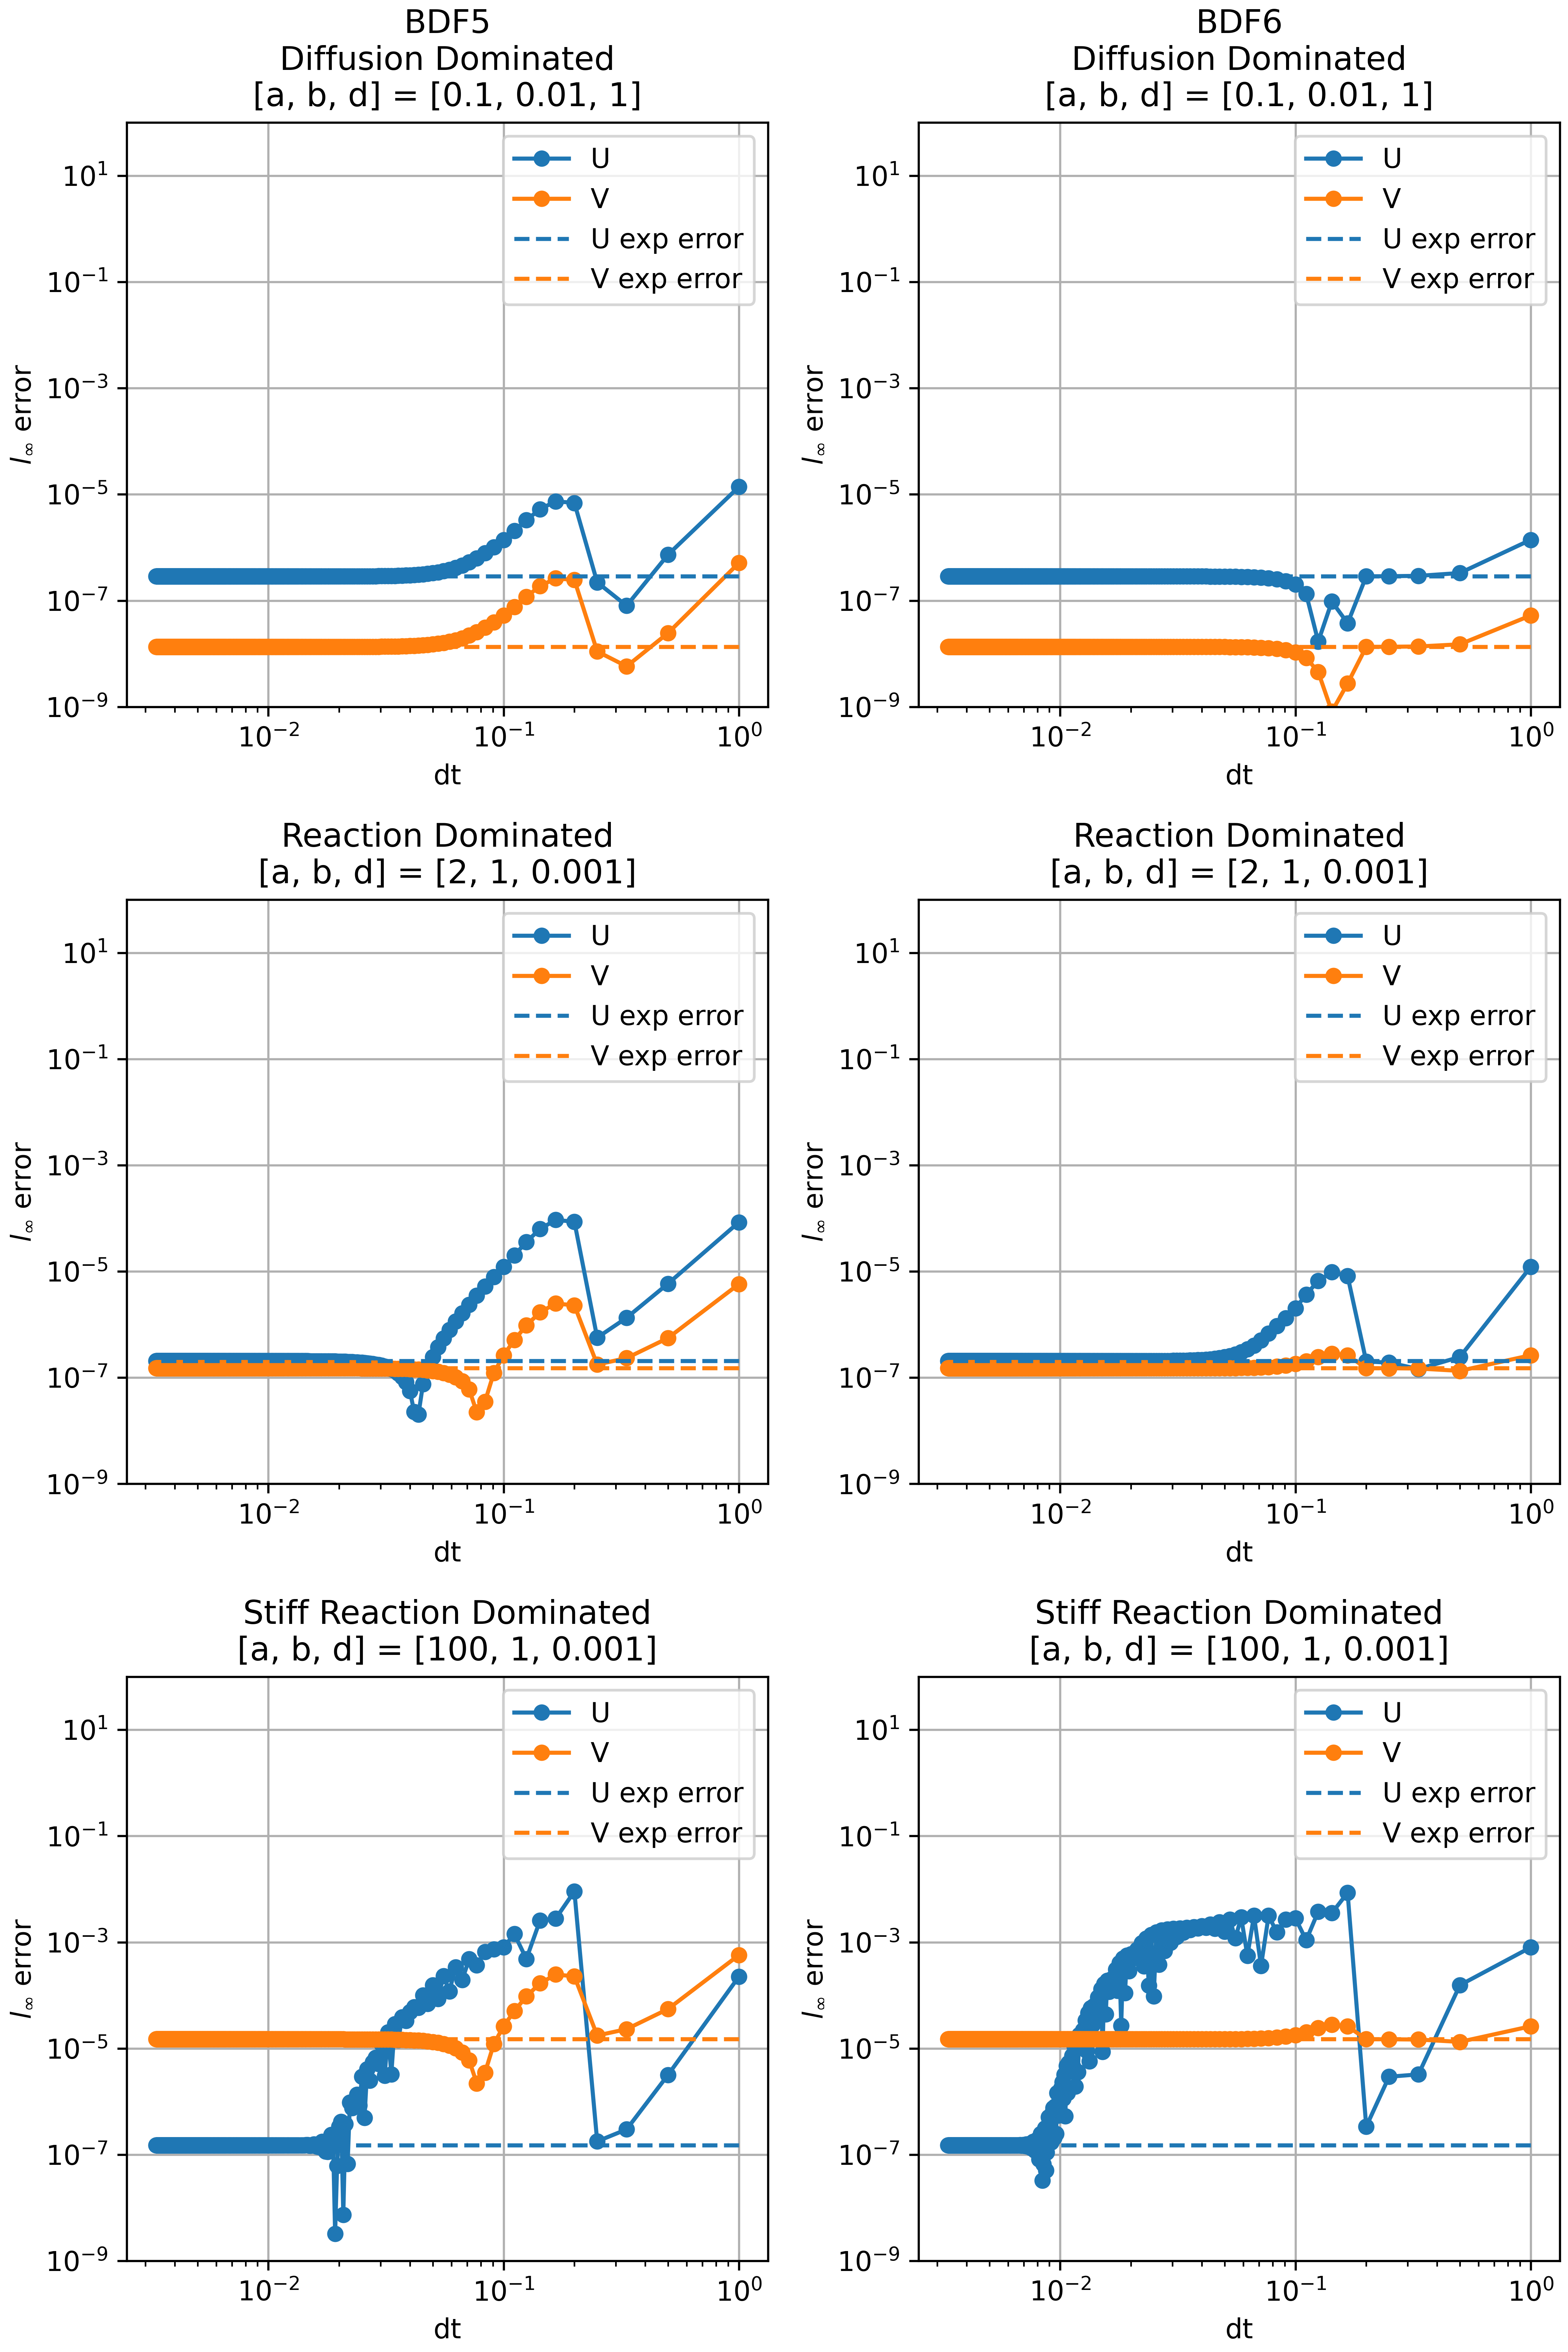
\includegraphics[width=5.75in]{images/BDF5BDF6problem2.png}\\
  \caption{BDF Solution for Problem 2 for Orders 5 and 6}
  \label{fig:errorProblem2BDF5and6}
\end{figure} 

\FloatBarrier


\subsection{Problem 3}
This problem examines a convection driven flow with the 6 neutron precursor groups shown in Equation \ref{eq:problem3}. Coefficients for system are shown in Table \ref{tab:problem3Coeffs}. 

\begin{equation}
\setlength{\jot}{15pt}
\begin{split}
    \frac{\partial \rho_{k}}{\partial t} = -v_{y}\frac{\partial \rho_{k}}{\partial y} - \lambda_{k}\rho_{k}& + \frac{M_{k}}{N_{A}}\gamma_{k}\Sigma_{f,k}\phi\sin\bigg(\frac{\pi}{L}\bigg), \quad k = 1, 2, \ldots 6
\end{split}
\label{eq:problem3}
\end{equation}

\noindent Each precursor has the same initial condition of zero and the source term for each precursor is scaled in the y-direction by the sine function and is applied in libowski using the mean value theorem. The source term comes from nuclear fission which typically follows a sine shape in the axial direction of a nuclear reactor. The spatial discretization is fixed at 50 cells for a 1 foot length of "pipe" in the y-direction. This make a small distance for the precursors to travel with a high velocity, creating a stiff system from the convective transport alone. Periodic boundary conditions are placed on the top and bottom of the solution domain, allowing the precursors to flow in an endless loop. The problem is ran for a total time of 1 second at which time, the solutions are compared to the solutions for Pad\'e method for a single time step of 1 second. Each of these Cauchy and BDF solvers are ran at various time steps then they are compared to the Pad\'e solution at 1 second. 

This problem was designed to induce very large imaginary parts for the eigenvalues ($\sim 100$), so that the Cauchy solvers can be well tested. These eigenvalues were manipulated by adding the periodic boundary conditions and by adjusting the ratio $v/dx$. As $v/dx \xrightarrow{} 0$ the imaginary part of the eigenvalues does as well.  


\begin{table}[b]
    \caption{\label{tab:problem3Coeffs} Coefficients used in the differential equations for problem 3}
    \centering
    %\begin{tabular}{c|p{1.5cm}|p{1.5cm}|p{1.5cm}|p{1.5cm}|p{1.5cm}|p{1.5cm}}
    \begin{tabular}{c|c|c|c}
    \hline
    Precursor Group & $v_{y}$(ft/s) &$\lambda $ (1/s) & $M_{k}\gamma_{k}\Sigma_{f,k}\phi/N_{A}$ (lbm/s/ft$^{3}$) \\
    \hline
    \hline
    1 & 2 & 0.0125 & 5.19E-02  \\  
    \hline
    2 & 2 & 0.0318 & 2.70E-01 \\  
    \hline
    3 & 2 & 0.109 & 2.62E-01 \\  
    \hline
    4 & 2 & 0.3170 & 7.47E-01 \\  
    \hline
    5 & 2 & 1.3500 & 2.17E-01 \\  
    \hline
    6 & 2 & 8.640  & 7.66E-02 \\  
    \hline
    \end{tabular}
\end{table}

Results from problem 3 are shown in Figure \ref{fig:problem3results}. These results are broken up into 4 plots. The top left hand plot is the error from each of the Cauchy and BDF solvers. Each of the other plots show the error of each of the Cauchy solvers on the complex plane along with a plot of the eigenvalues for the problem at each time step. From each of these three plots, you can see that the eigenvalues are scaled by the size of the time step taken so solve the problem. Just like in problem 1, this shows that problems with "bad" eigenvalues can be scaled down to increase the accuracy of Cauchy solvers. 

From Figure \ref{fig:problem3results}, error from Cauchy solvers decrease at a faster rate than the BDF solvers. While the Cauchy solvers get lower error, they never fully converge to the Pad\'e solution, which is used as the goal solution. What is very interesting about the Cauchy solvers is which ones approaches closest to the goal solution. In theory the Hyperbolic and Parabolic solvers should be the best, in that order. This is because each of these solvers has a wider range of accuracy on the imaginary plane. However, the Parabolic solver is about an order of magnitude worse error than the Hyperbolic and CRAM solvers. Again, like the previous problems, the Hyperbolic solver works the best with systems with "bad" eigenvalues. 

Like the previous problems, the exponential solvers outperformed the BDF methods. Even with a system that imposes increased error from the Cauchy solvers, the BDF solvers could not compete with the accuracy of the exponential solvers. What is important to note is that while each method obtains increased accuracy from reducing the time step size, they achieve this accuracy from different mathematical aspects. BDF solvers increase their accuracy by the traditional method of approaching the actual derivative by reducing the time step size. Cauchy methods increase their accuracy by manipulating properties of the system of ODE's and closing the spread of their eigenvalues. 


\FloatBarrier

\begin{sidewaysfigure}[t]
  \centering
  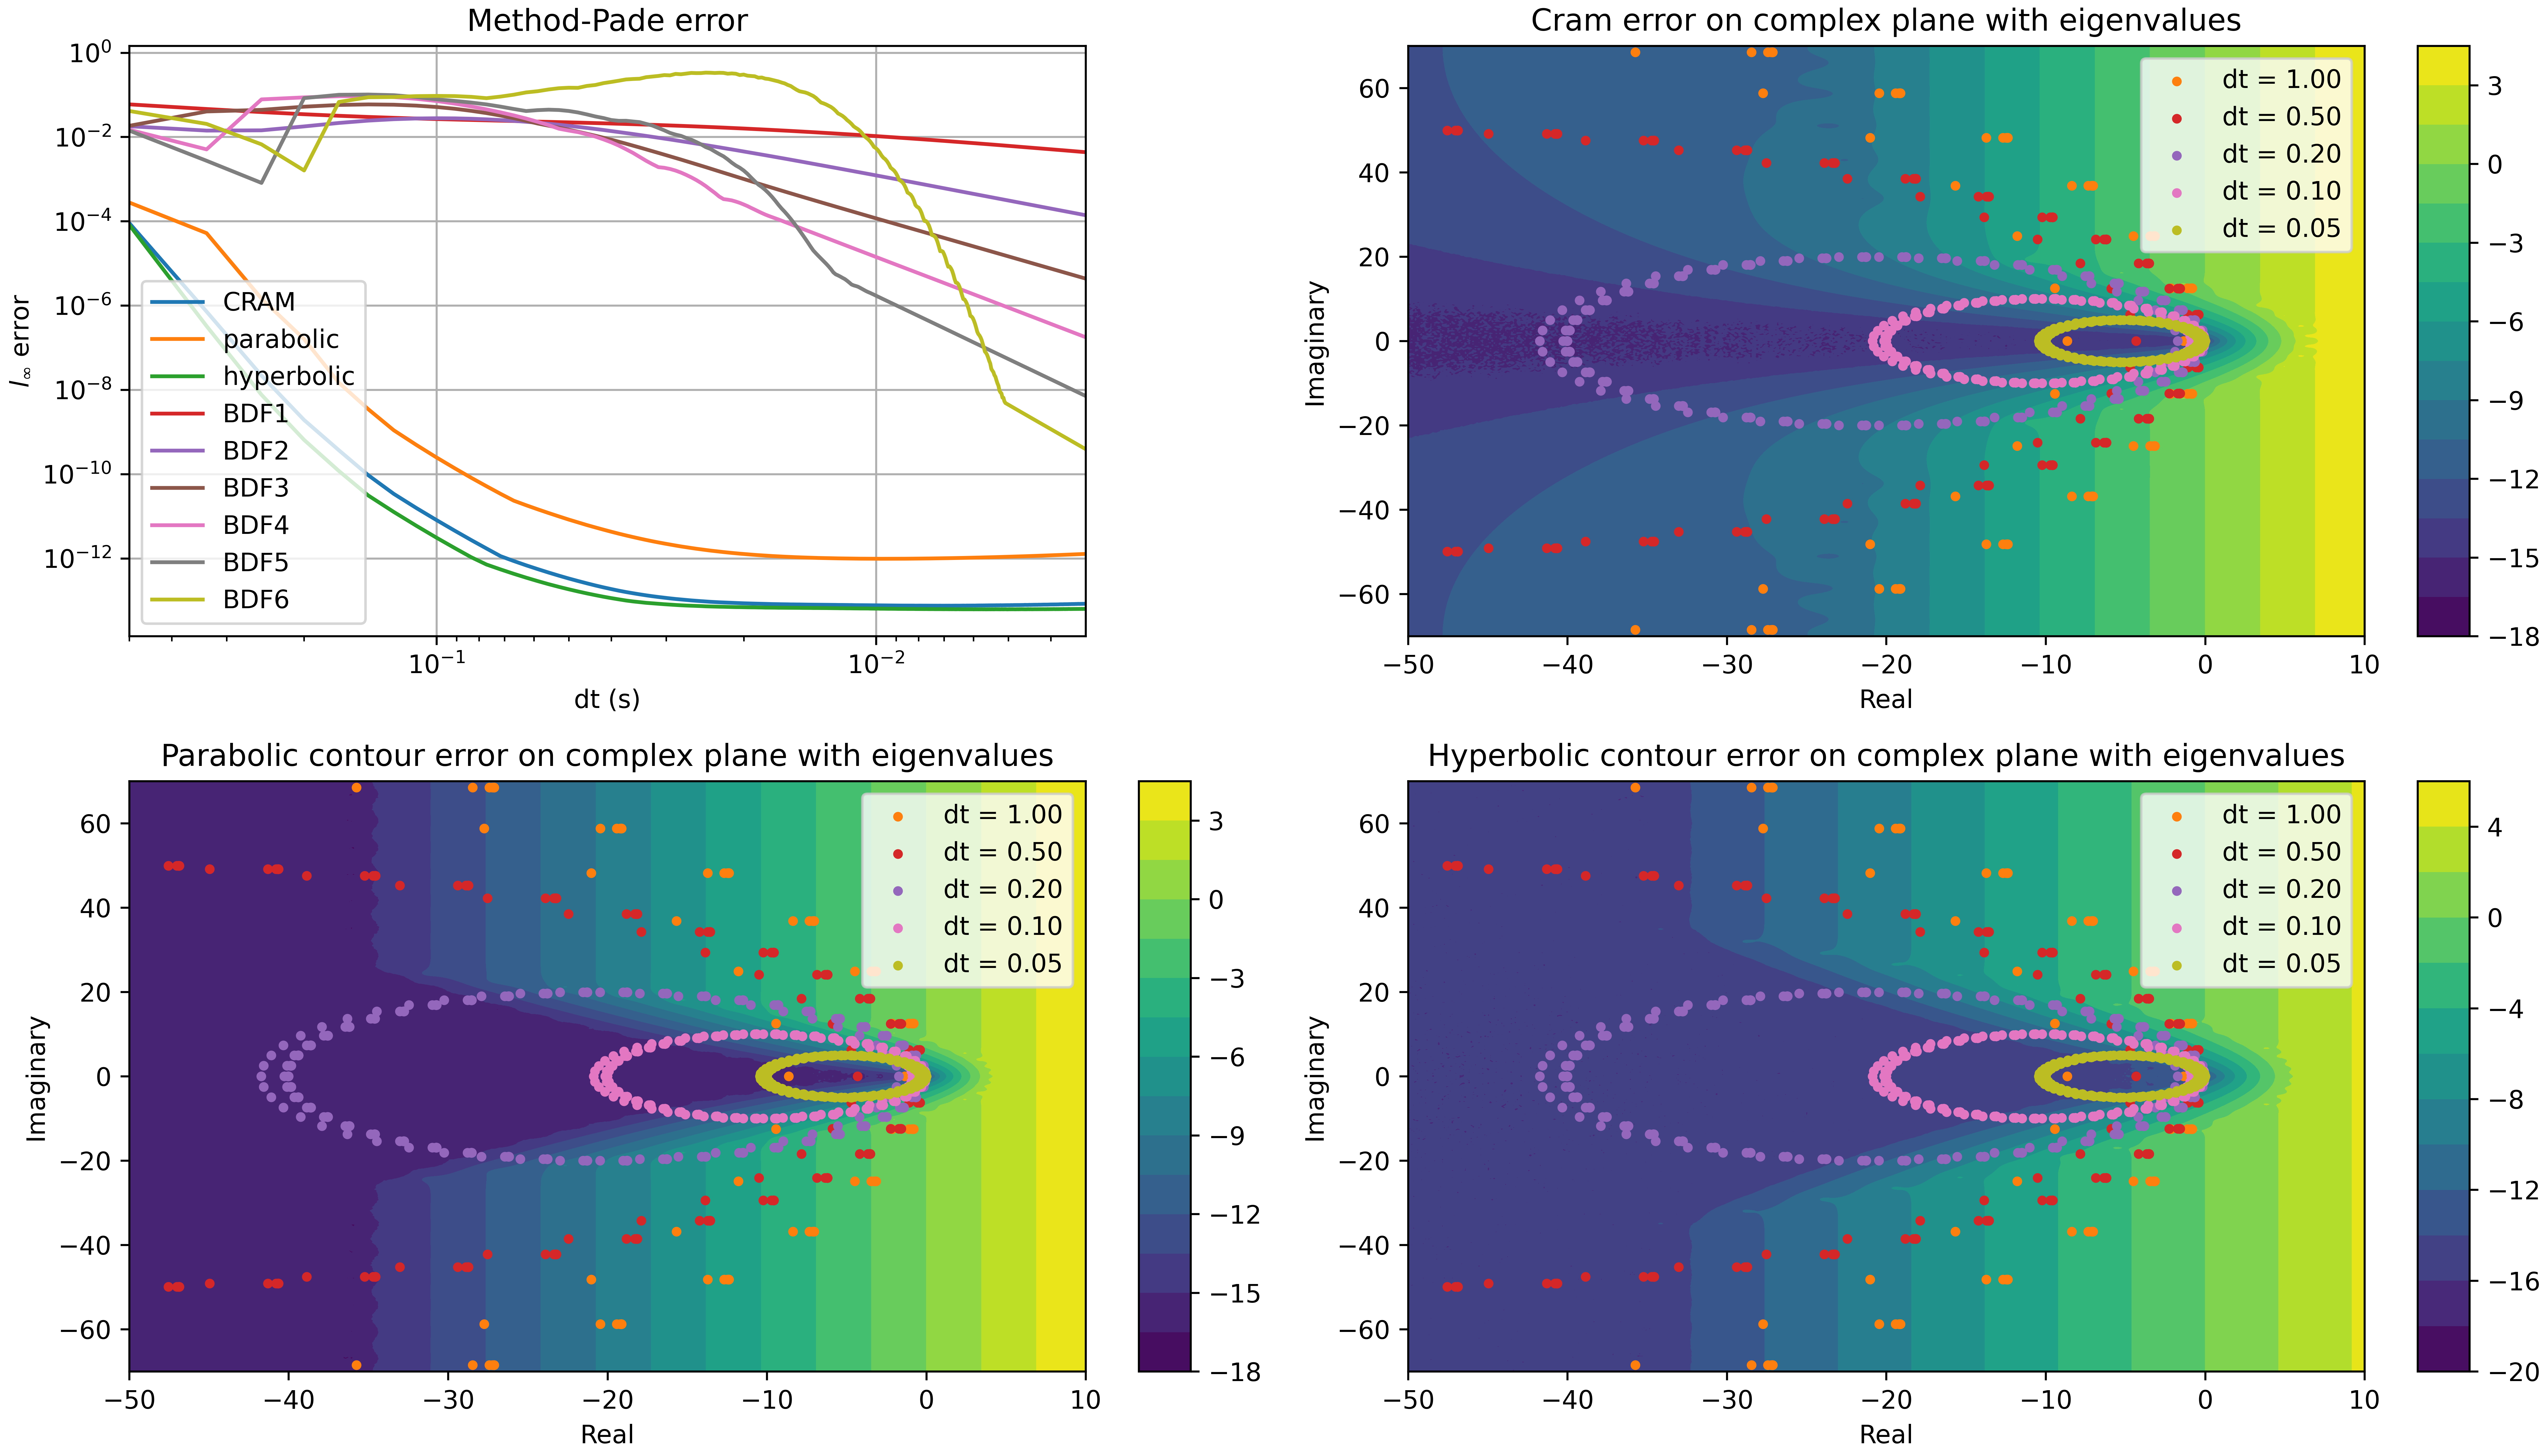
\includegraphics[width=9in]{images/problem3results.png}\\
  \caption{Cauchy solver results for problem 3}
  \label{fig:problem3results}
\end{sidewaysfigure} 
